\documentclass[11pt]{article}

\usepackage{sectsty}
\usepackage{graphicx}
\usepackage{multirow}
\usepackage[left= 2cm]{geometry}


\title{ Gestion de Asignaturas}
\author{ Quintero Angelica, Zambrano Pianina, Ramos Jurany, Ayoví Leah, Añapa Alex, Ulloa Alber }
\date{\today}

\begin{document}
\maketitle	
\section{Introduccion}

En respuesta a las demandas cada vez más complejas del
entorno educativo actual, presentamos un software de gestión de
asignaturas que simplifica y potencia la administración de
programas académicos. En un mundo educativo en constante
evolución, la gestión de asignaturas se ha vuelto esencial
para el éxito de las instituciones educativas y laexperiencia 
de aprendizaje de los estudiantes. Este software surge como
una solución integral para abordar el desafío crítico de la 
gestión de asignaturas, un tema de gran relevancia en la
educación contemporánea.


La necesidad de una plataforma que simplifique desde la
planificación curricular hasta la comunicación y
evaluación se vuelve cada vez más evidente. Este software se
destaca por su capacidad para centralizar la información
y la comunicación, permitiendo a educadores y estudiantes
interactuar de manera efectiva a través de una interfaz
intuitiva. Además, ofrece una amplia gama de herramientas
analíticas que permiten un seguimiento detallado del progreso
académico de los estudiantes y la identificación de áreas de
mejora. En este texto, exploraremos cómo este
software revoluciona la forma en que se gestionan las
asignaturas, presentando sus características clave y
discutiendo
cómo aborda los desafíos actuales en la educación. Esto
preparará el terreno para comprender en detalle las ventajas y
beneficios que ofrece en el ámbito educativo, allanando el
camino hacia una administración más efectiva y una
experiencia de aprendizaje enriquecida.
\section{Objetivo General}

El objetivo general de este estudio es analizar y demostrar
cómo el software de gestión de asignaturas presentado en
estetexto
revoluciona la administración de programas académicos en el
entorno educativo contemporáneo. Para lograr este propósito,
se llevará a
cabo una investigación exhaustiva que se centrará en las
características clave de esta plataforma, su capacidad para
simplificar laplanificación curricular, mejorar la
comunicación entre educadores y estudiantes, y proporcionar
herramientas analíticas avanzadas parael seguimiento del
progreso académico. Además, se explorarán los desafíos
actuales en la educación que este software aborda de manera
efectiva. El resultado final de esta investigación será
proporcionar una comprensión sólida y detallada de las
ventajas y beneficios que esta solución ofrece en el ámbito
educativo, con el objetivo de contribuir a una administración
más efectiva de los programas académicos y enriquecer la
experiencia de aprendizaje de los estudiantes.


\section{Objetivos Especificos}
\begin{enumerate}
\item Evaluar la capacidad del software de gestión de
asignaturas para simplificar la planificación
curricular:

*Analizar cómo el software facilita la creación de
programas académicos, horarios y asignación de recursos
educativos.

*Medir la eficiencia y efectividad del software en la
organización de planes de estudio, tareas
administrativas y gestión de recursos.

*Identificar las características específicas del
software que contribuyen a la simplificación de la
planificación curricular.

\item Examinar cómo el software mejora la comunicación entre educadores y estudiantes:

*Investigar cómo la plataforma facilita la interacción
entre docentes y alumnos, incluyendo la comunicación en
tiempo real y la colaboración en línea.

*Evaluar cómo el software contribuye a la transparencia
en la comunicación, permitiendo un seguimiento más 
cercano del progreso estudiantil.

*Identificar las herramientas de comunicación clave del
software y su impacto en la experiencia de aprendizaje.

\item Analizar las herramientas analíticas del software
para el seguimiento del progreso académico:

*Examinar las capacidades analíticas del software para
recopilar y procesar datos sobre el rendimiento
estudiantil.

*Evaluar la generación de informes y análisis de datos
proporcionados por el software.

*Determinar cómo estas herramientas ayudan a los
educadores a identificar áreas de mejora y tomar
decisiones informadas.

\item Explorar cómo el software aborda los desafíos
actuales en la educación:

*Identificar los desafíos comunes en la administración
académica y la experiencia de aprendizaje en el entorno
educativo actual.


*Analizar cómo el software aborda específicamente estos
desafíos, como la optimización de recursos, la
adaptación a entornos de
aprendizaje en línea y la gestión eficaz de datos.

*Comparar las soluciones propuestas por el software con
las prácticas tradicionales de gestión académica.

\item Presentar una comprensión detallada de las
ventajas y beneficios del software en el ámbito
educativo:

*Resumir de manera integral las ventajas clave del
software en términos de eficiencia administrativa,
mejora del rendimiento estudiantil y experiencia de
aprendizaje enriquecida.


*Destacar los beneficios específicos para educadores,
administradores escolares y estudiantes.


*Proporcionar ejemplos concretos y casos de uso que
ilustren cómo el software puede transformar la gestión
de asignaturas en
instituciones educativas. 
\end{enumerate}
\section{Modelo del sistema}
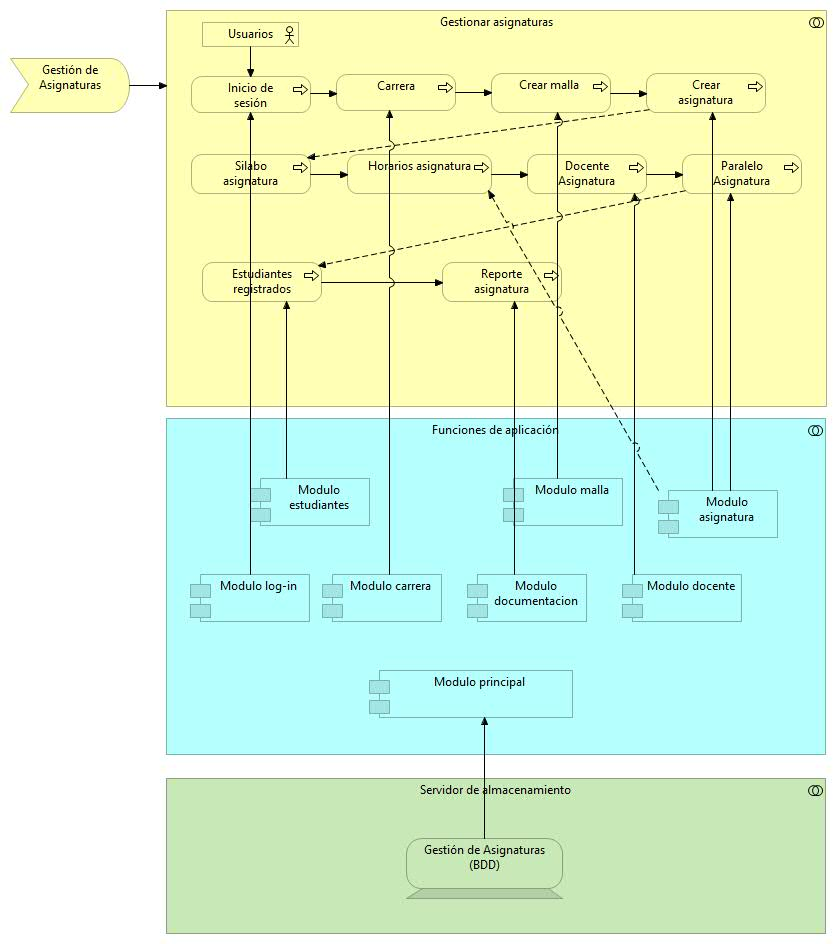
\includegraphics[scale=0.55]{ModelG.A.jpg}
\section{Prototipo}
\section{Prototipo}

\includegraphics[scale=0.40]{0.png}
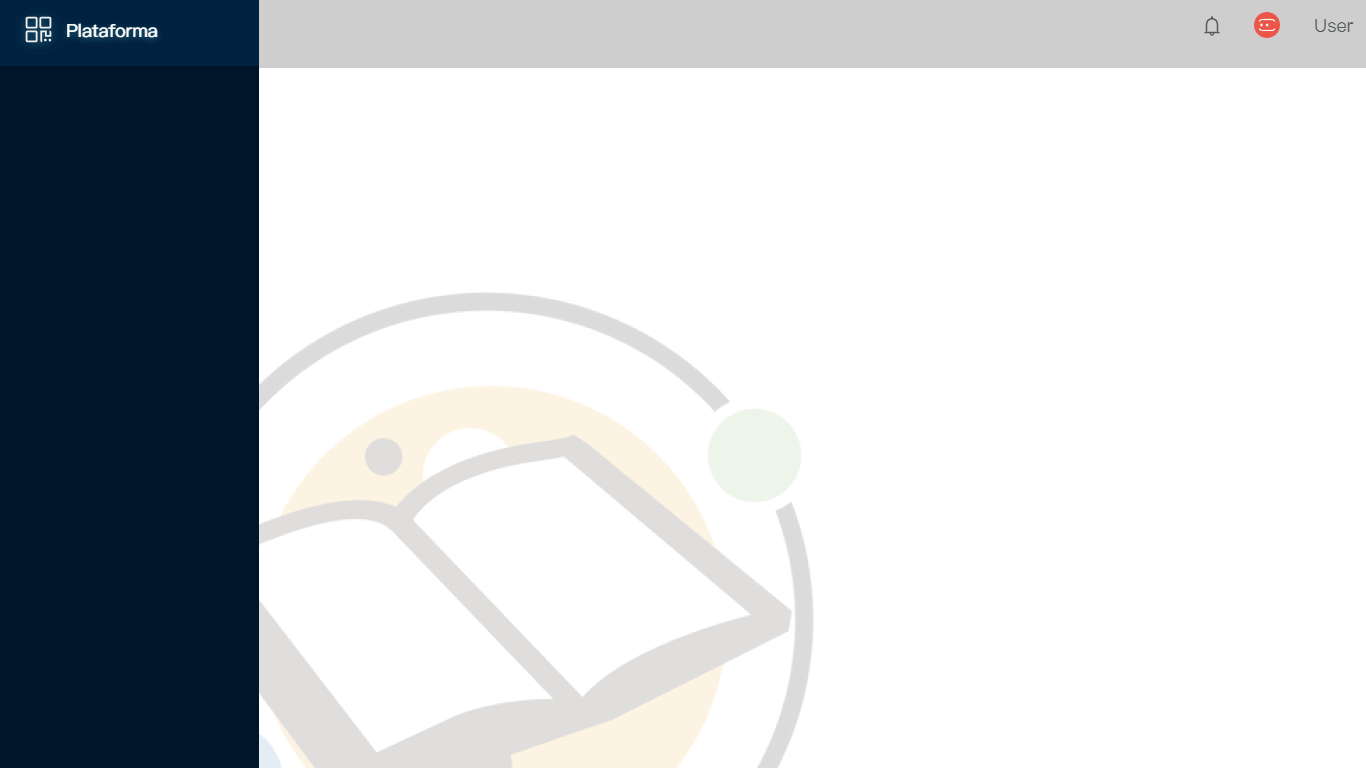
\includegraphics[scale=0.40]{1.png}
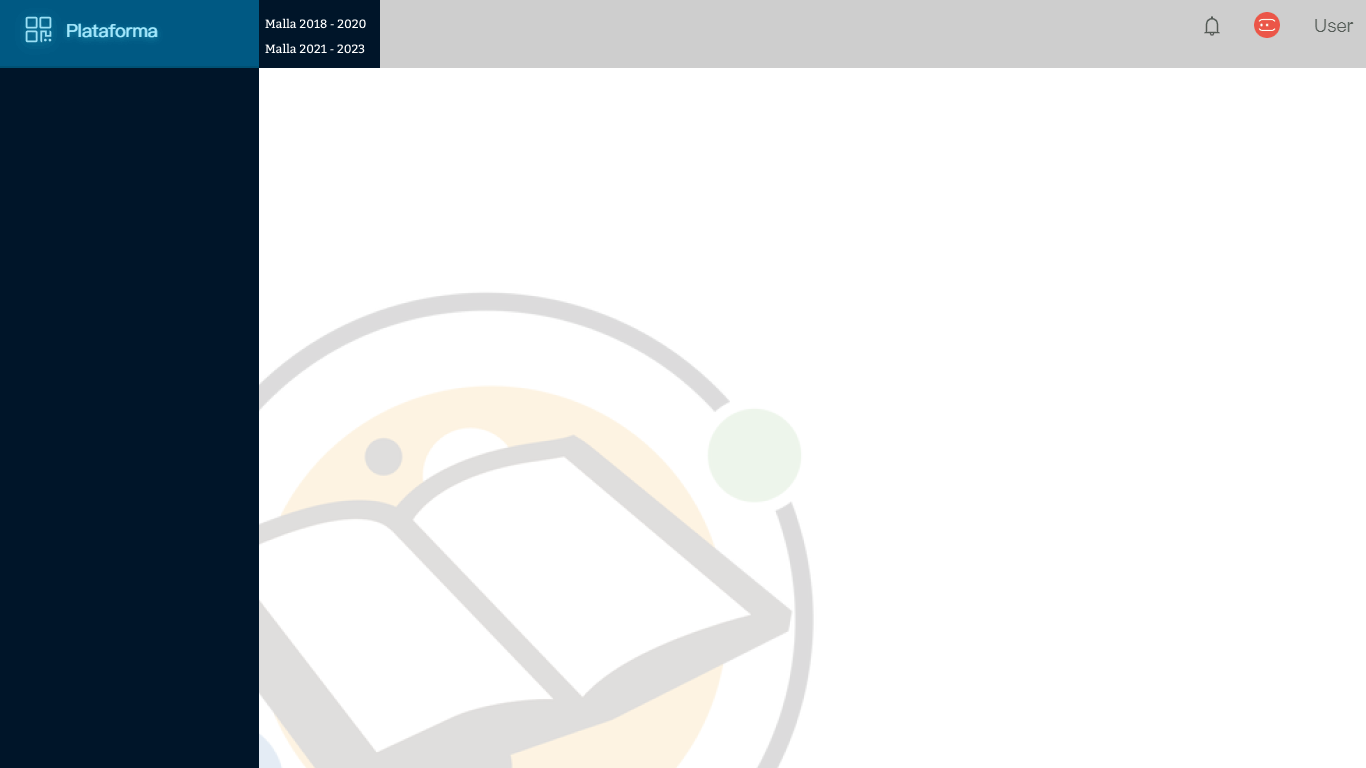
\includegraphics[scale=0.40]{2.png}
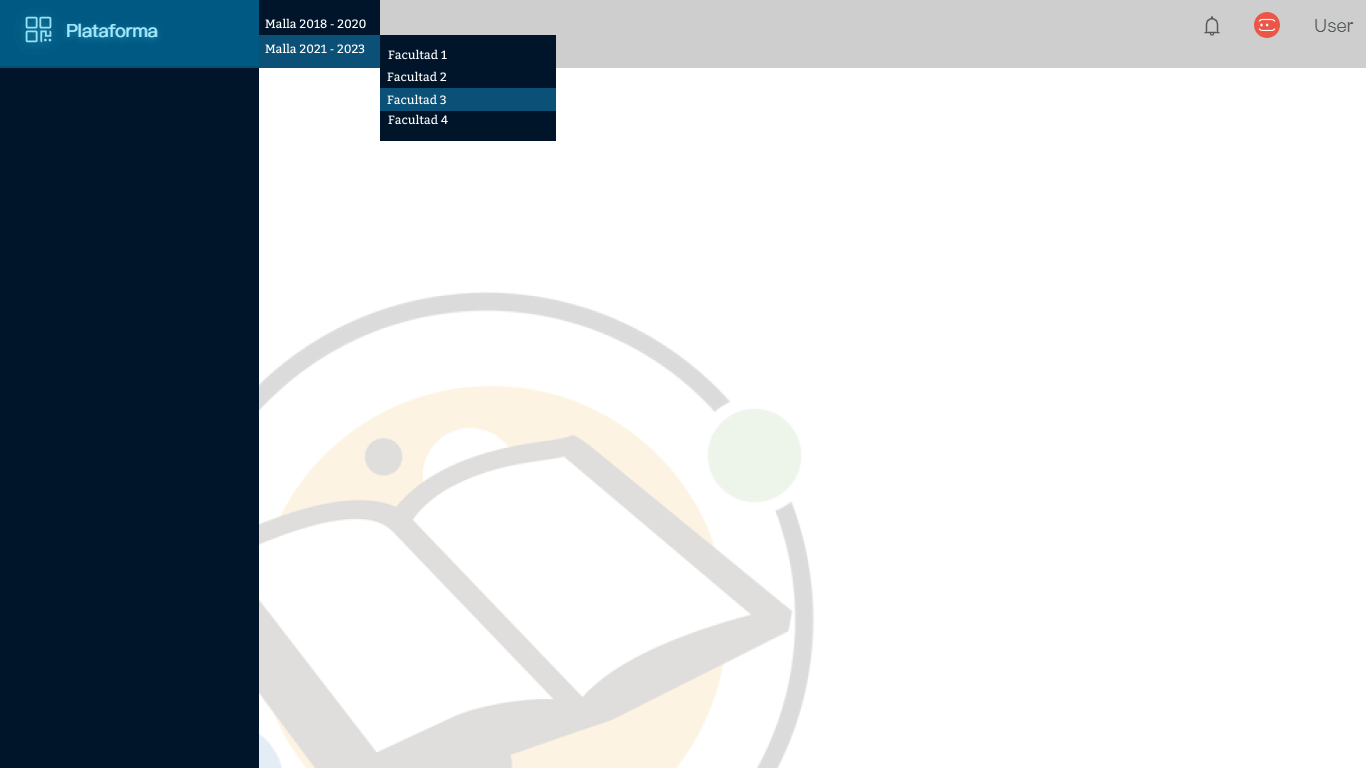
\includegraphics[scale=0.40]{3.png}
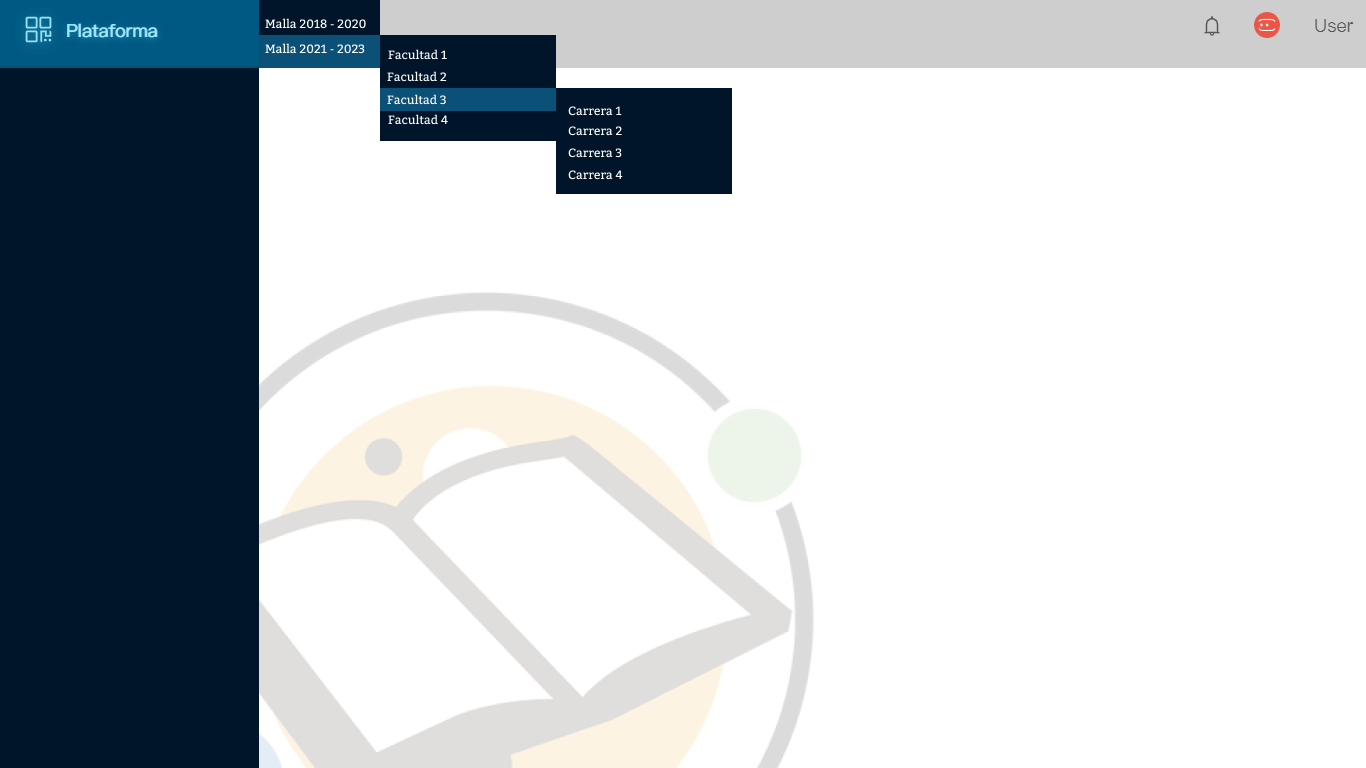
\includegraphics[scale=0.40]{4.png}
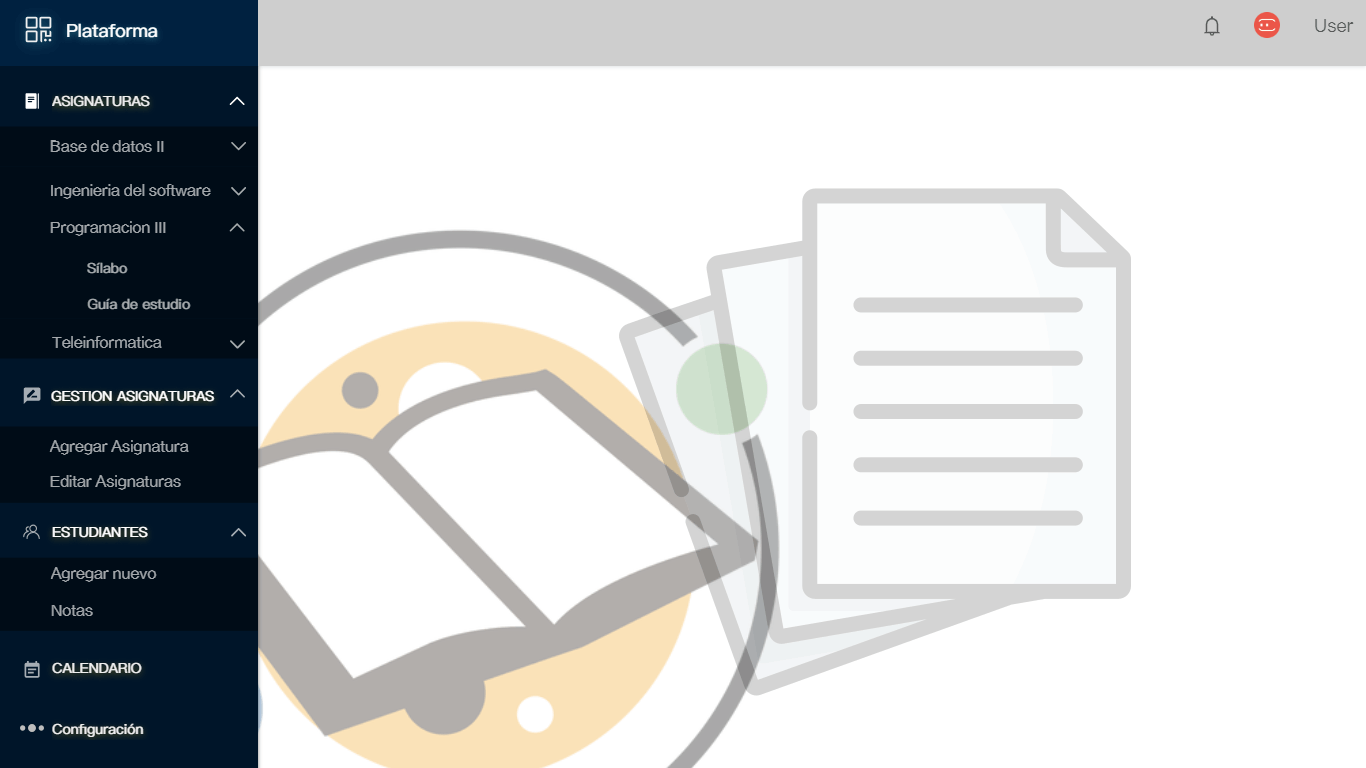
\includegraphics[scale=0.40]{5.png}
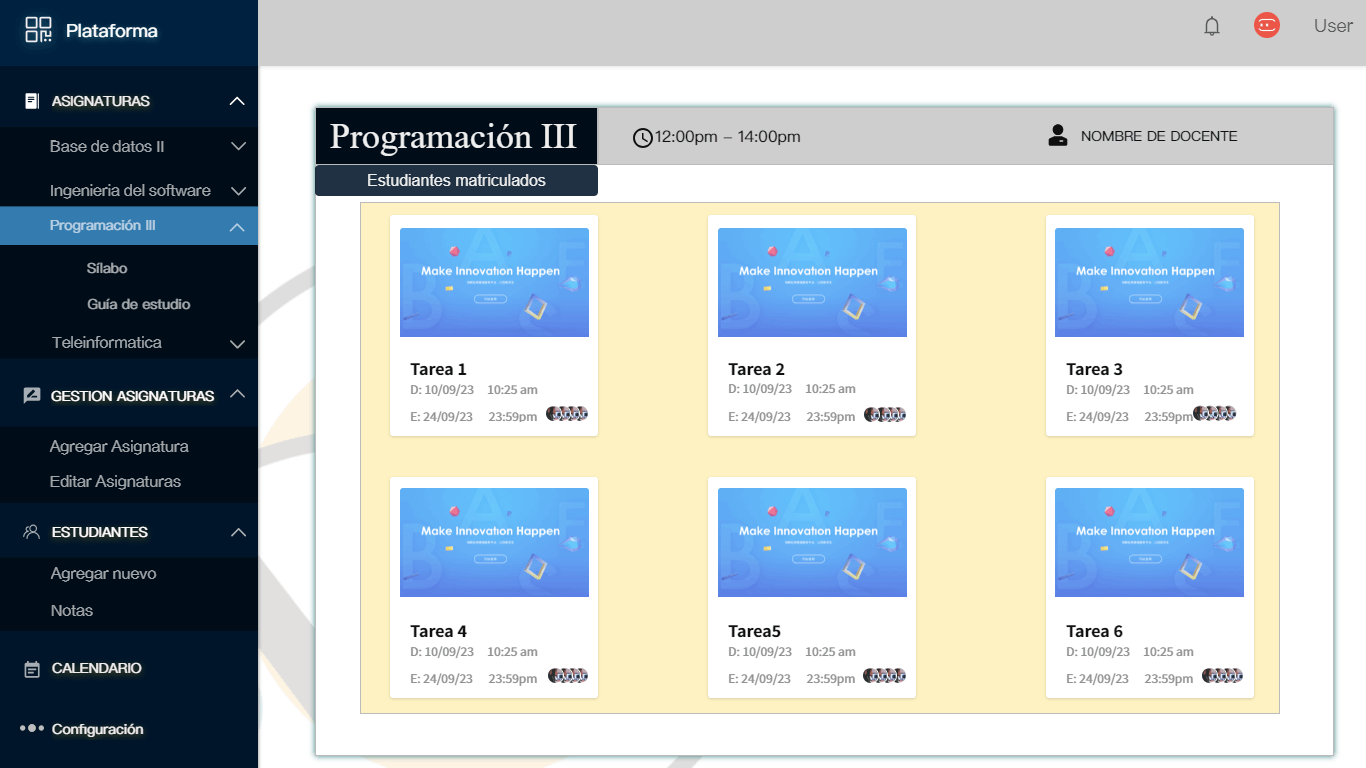
\includegraphics[scale=0.40]{6.png}
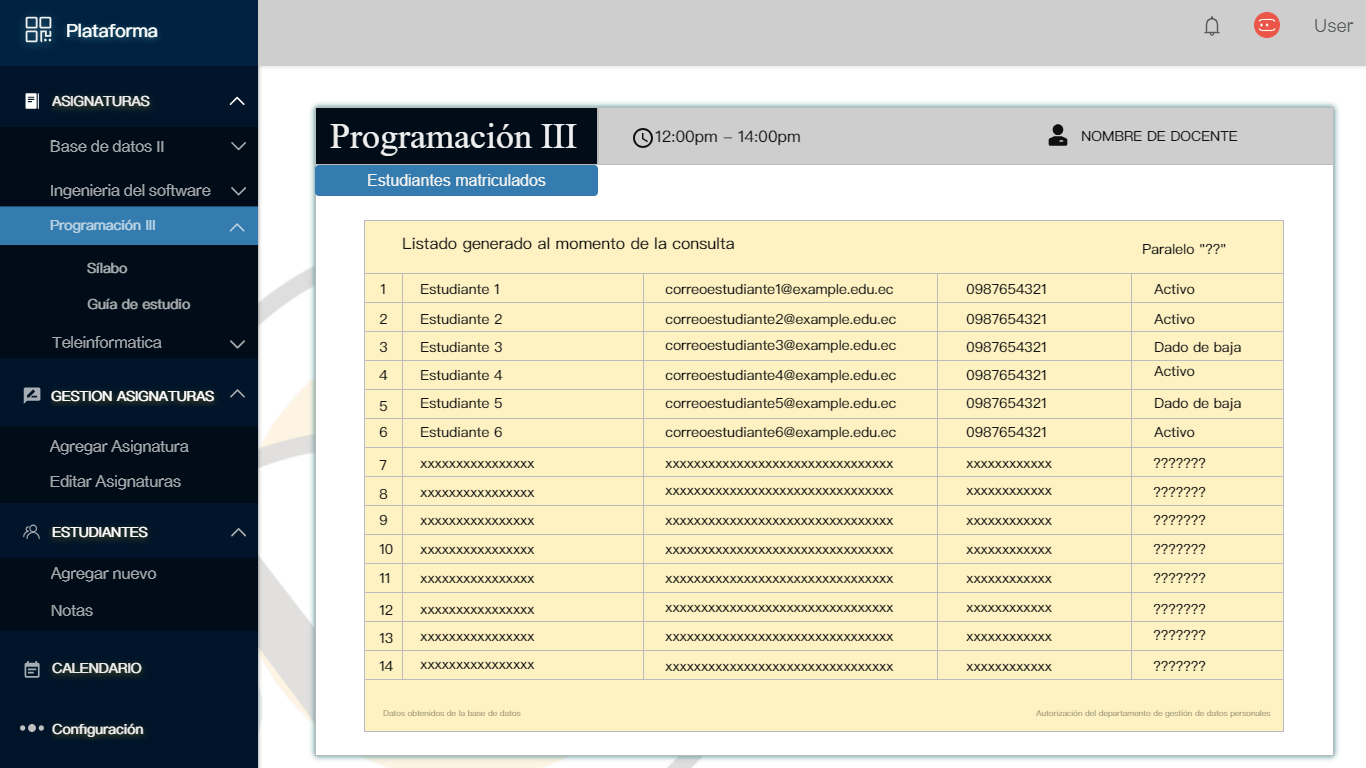
\includegraphics[scale=0.40]{7.png}
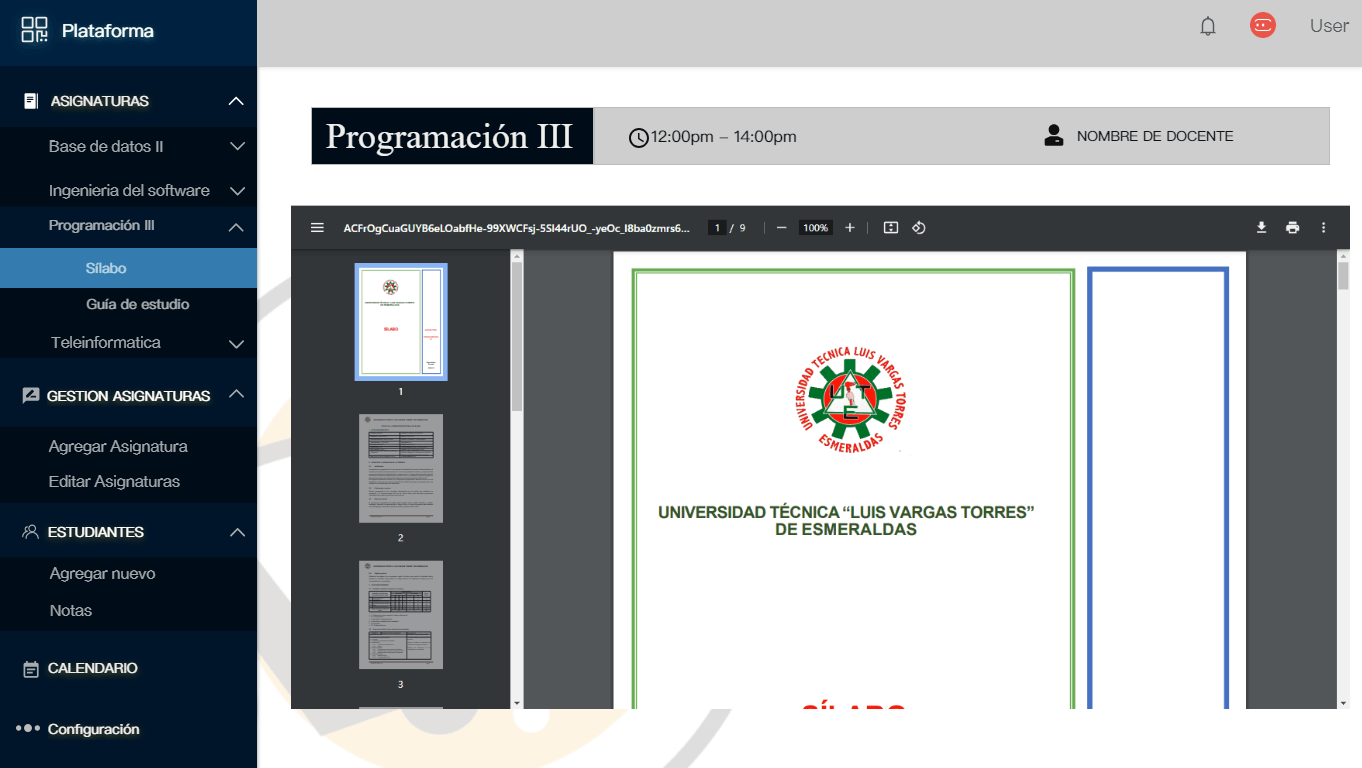
\includegraphics[scale=0.55]{8.png}
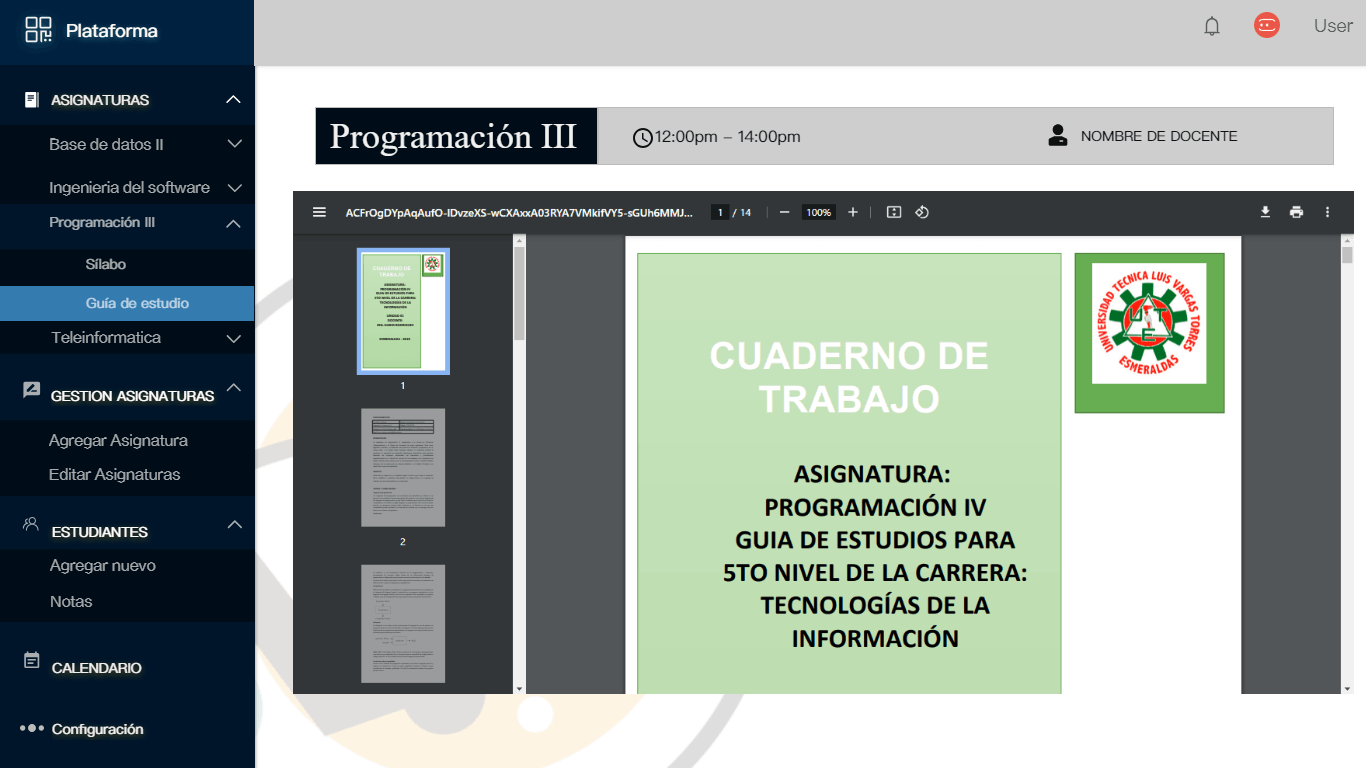
\includegraphics[scale=0.40]{9.png}
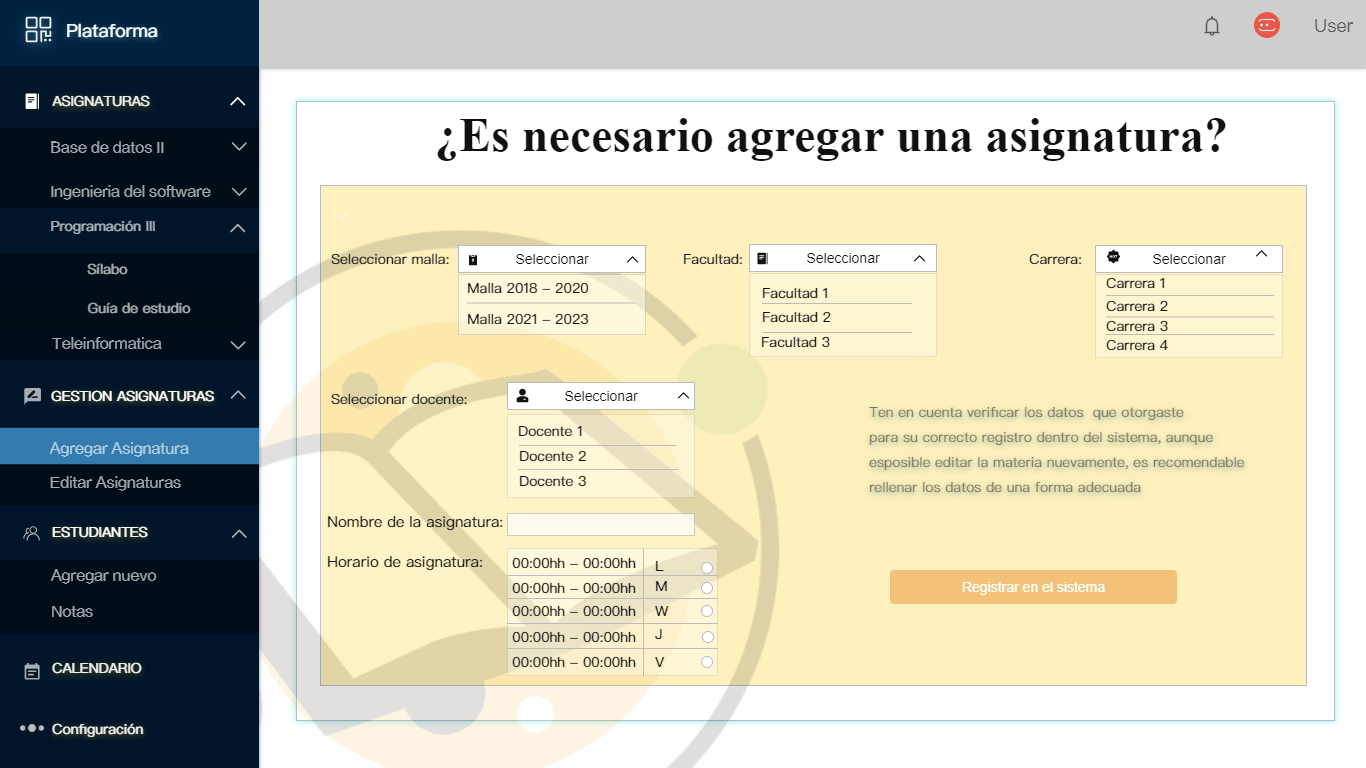
\includegraphics[scale=0.40]{10.png}
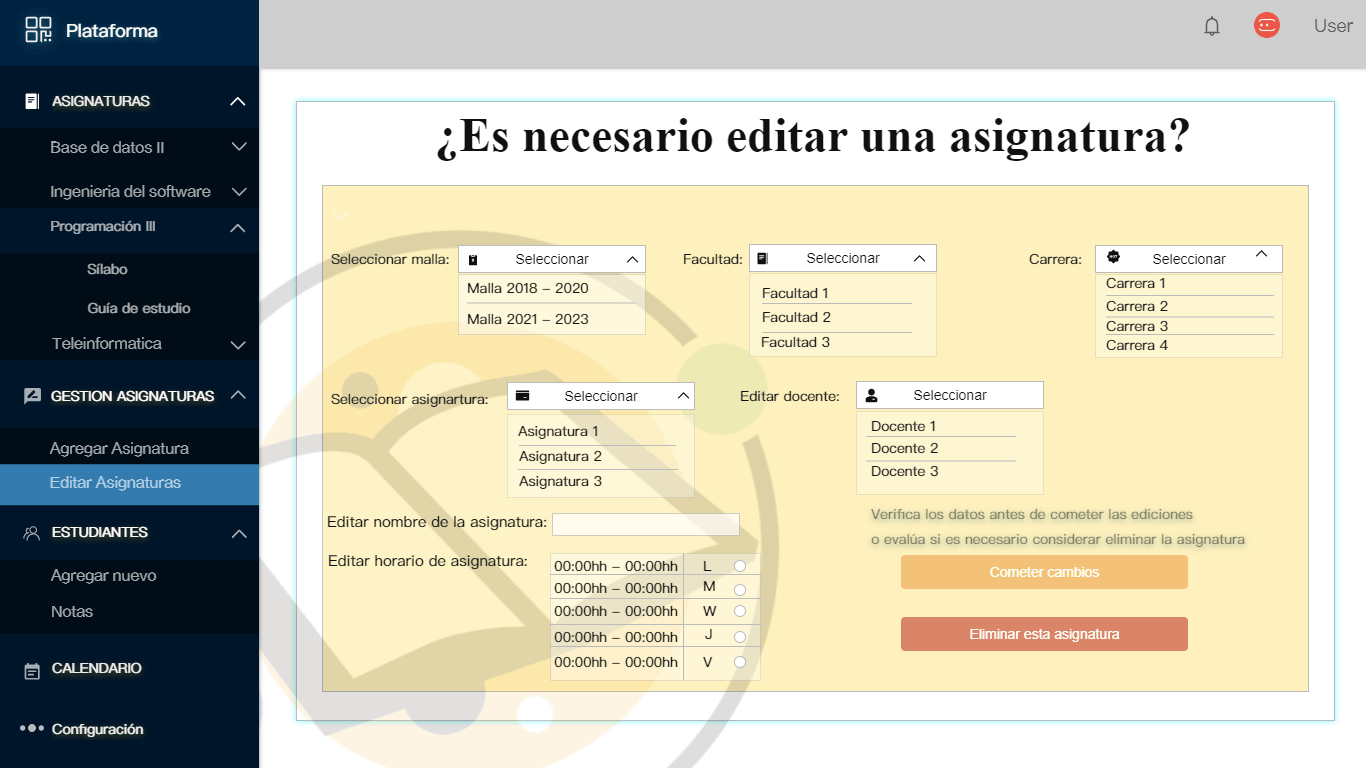
\includegraphics[scale=0.40]{11.png}
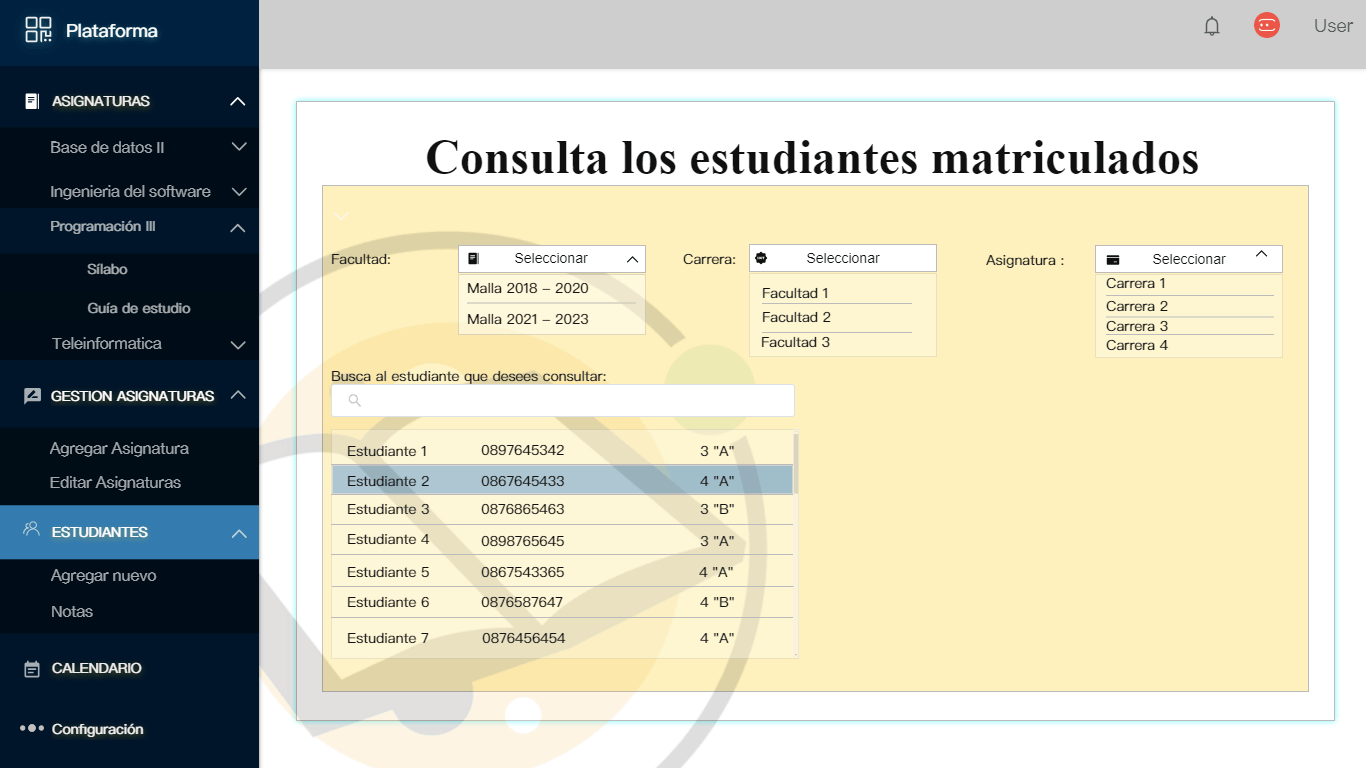
\includegraphics[scale=0.40]{12.png}
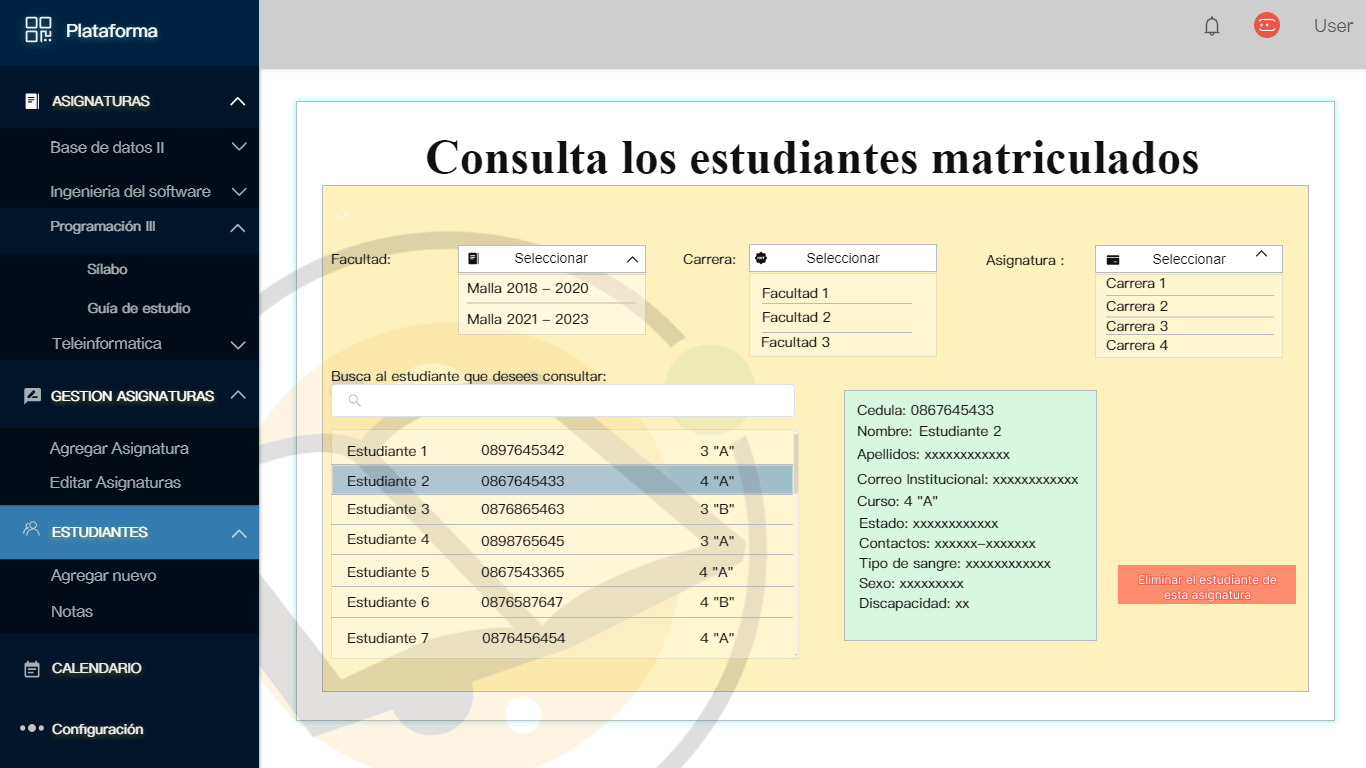
\includegraphics[scale=0.40]{13.png}
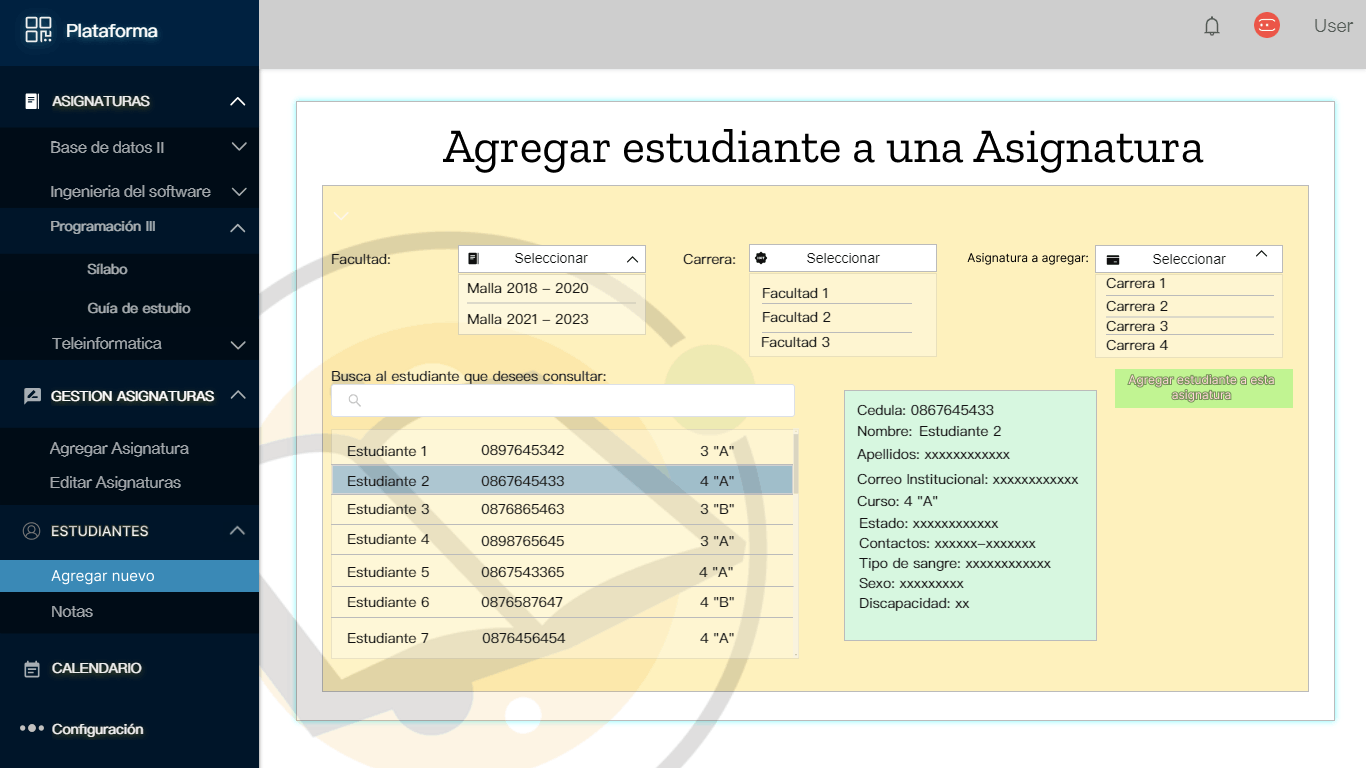
\includegraphics[scale=0.40]{14.png}
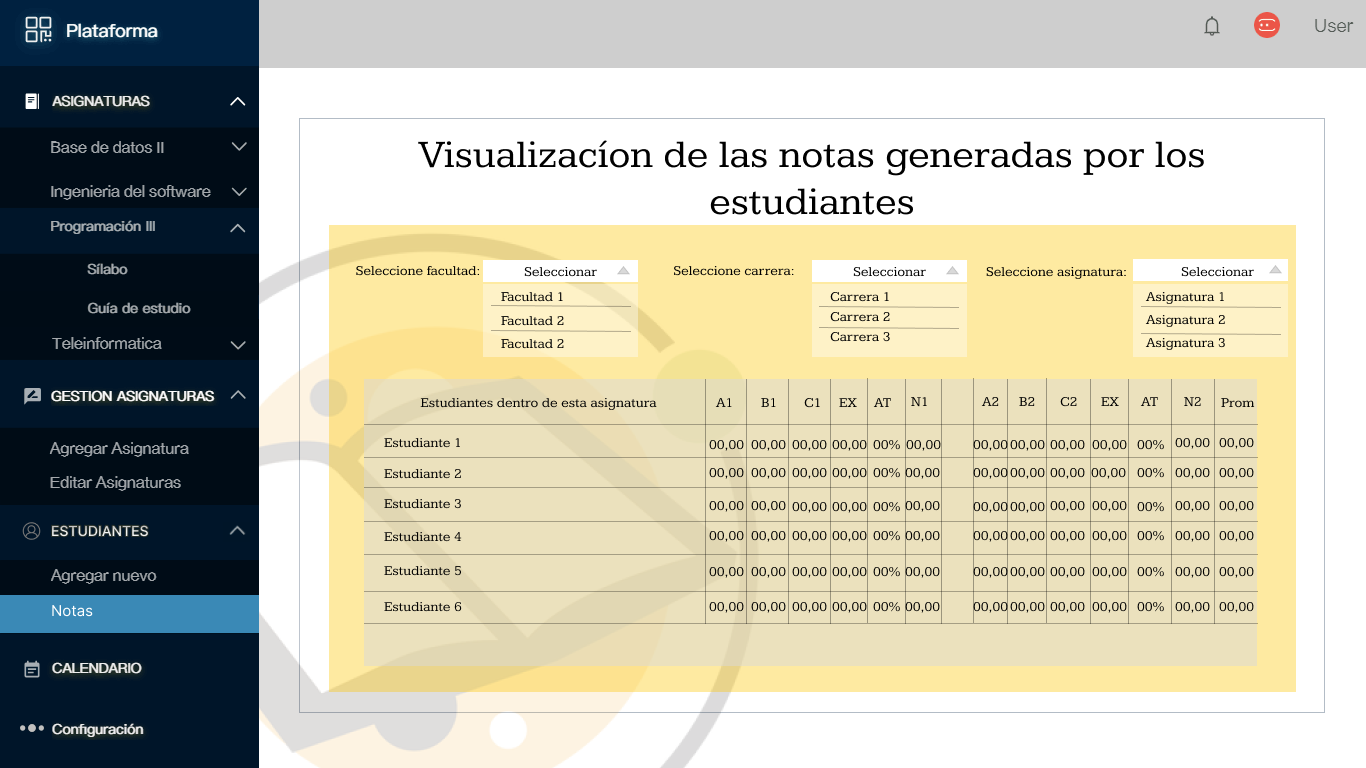
\includegraphics[scale=0.40]{15.png}
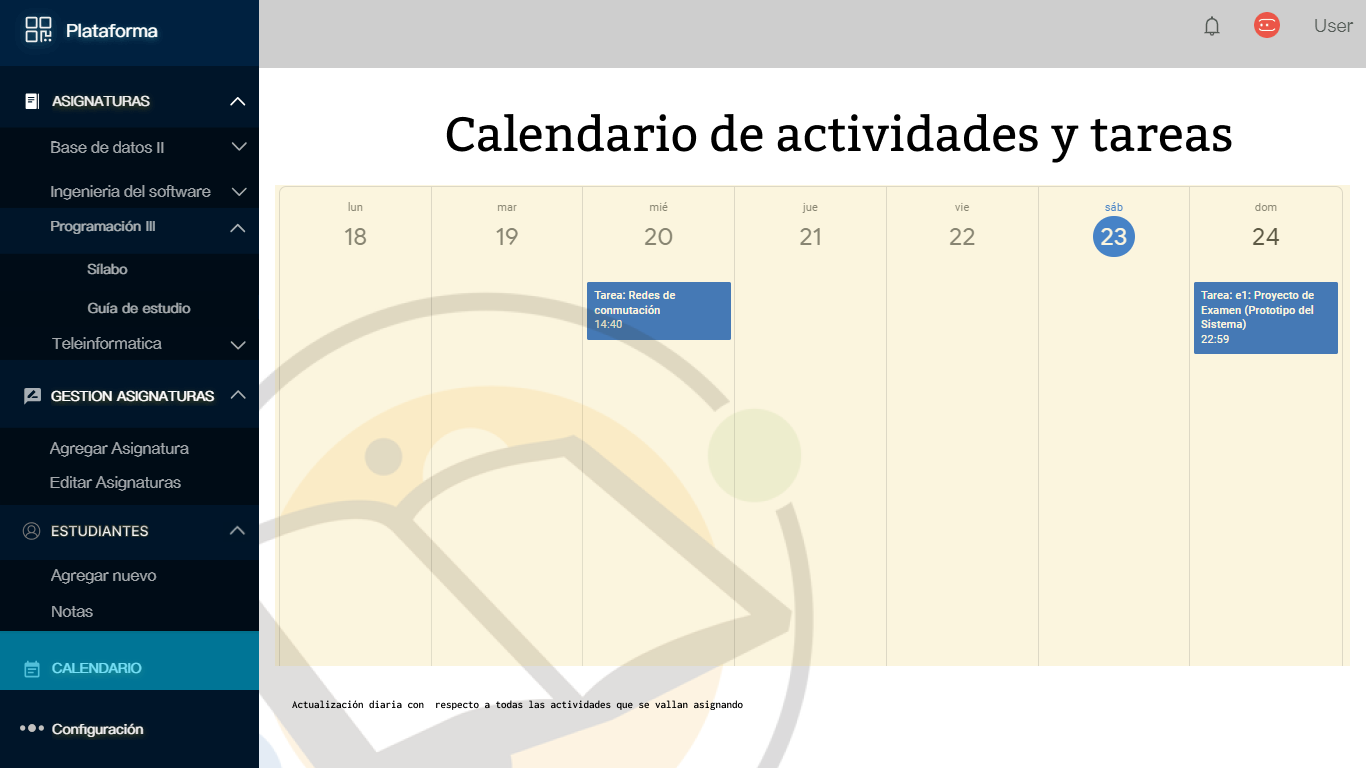
\includegraphics[scale=0.40]{16.png}
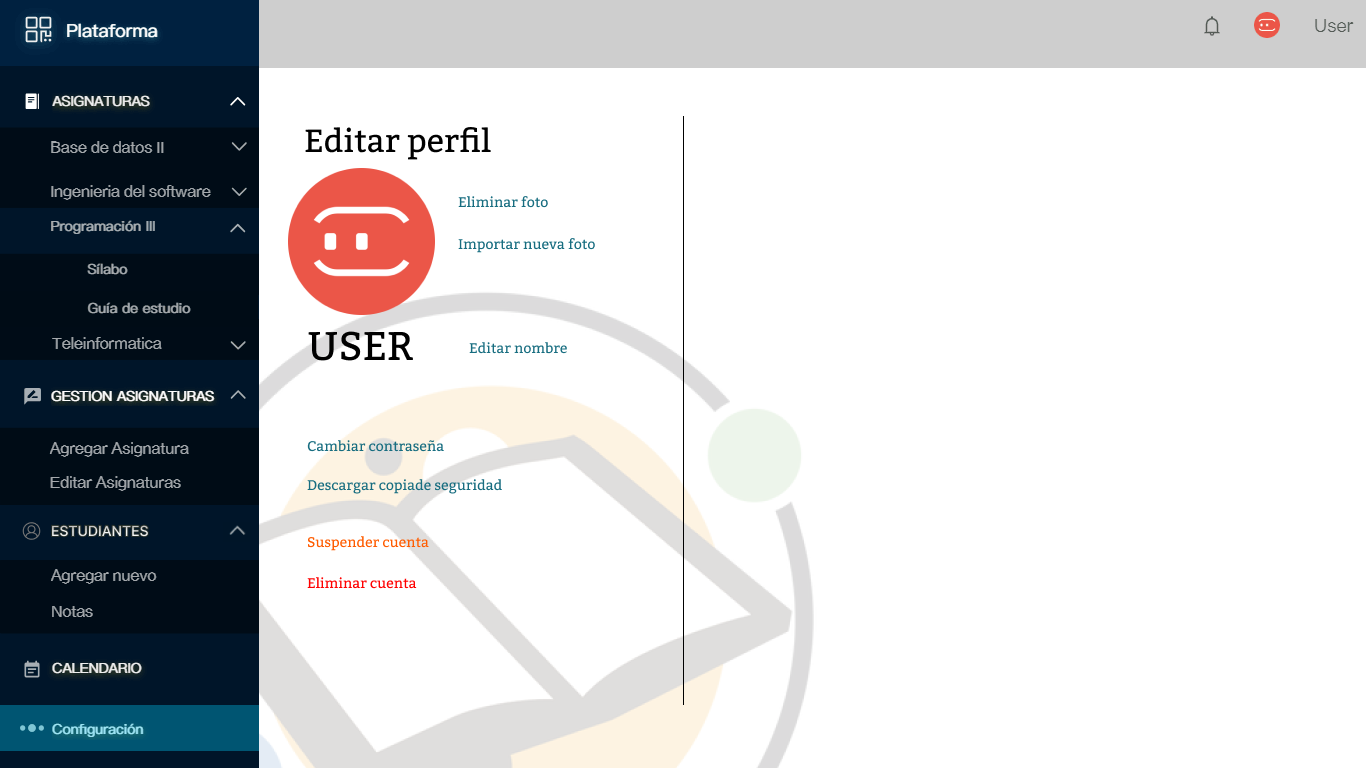
\includegraphics[scale=0.40]{17.png}
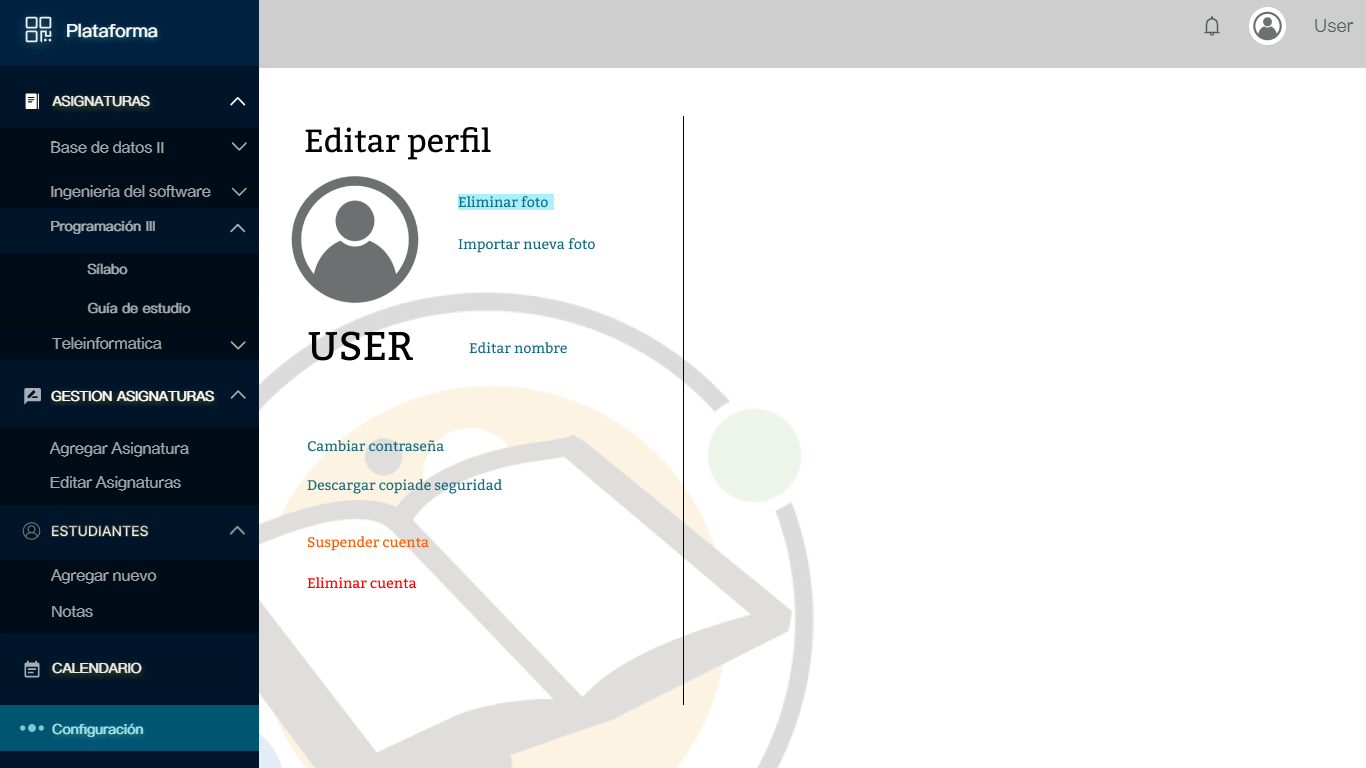
\includegraphics[scale=0.40]{18.png}
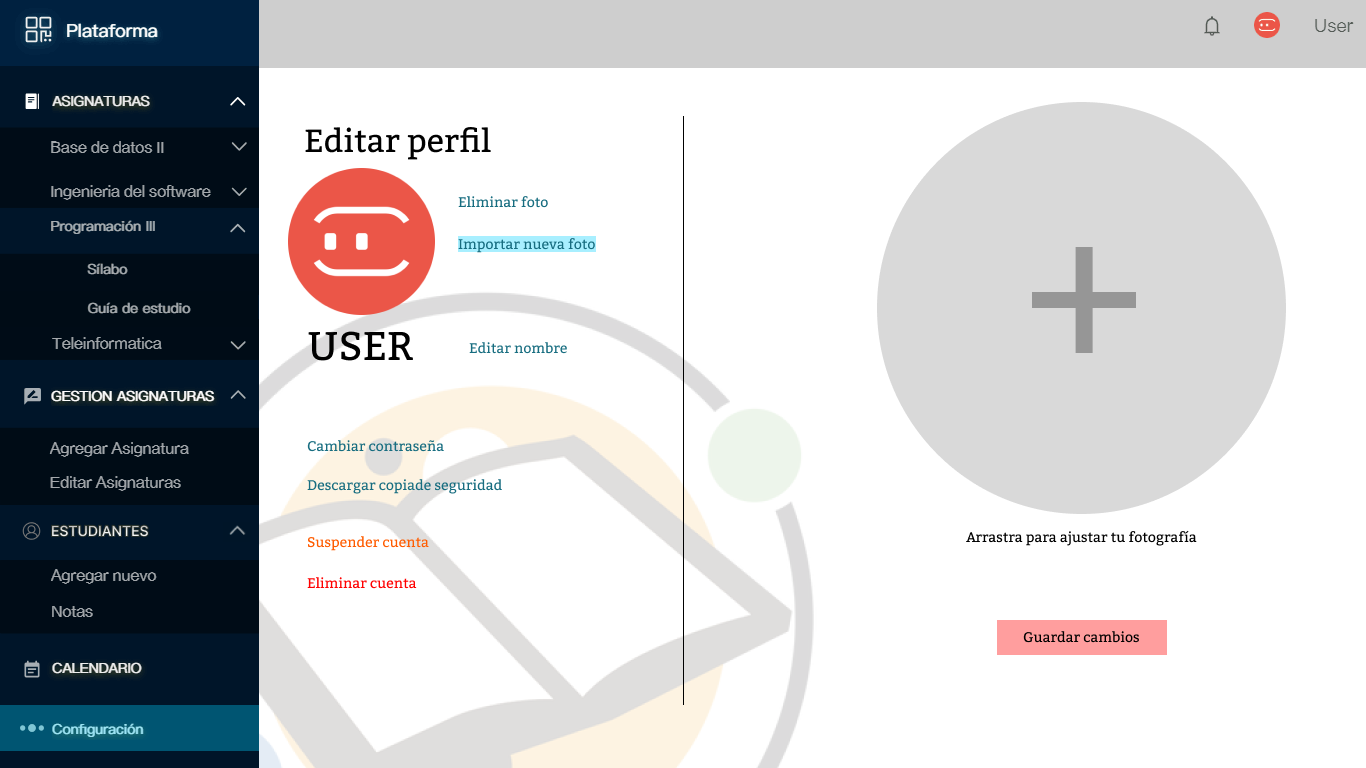
\includegraphics[scale=0.40]{19.png}
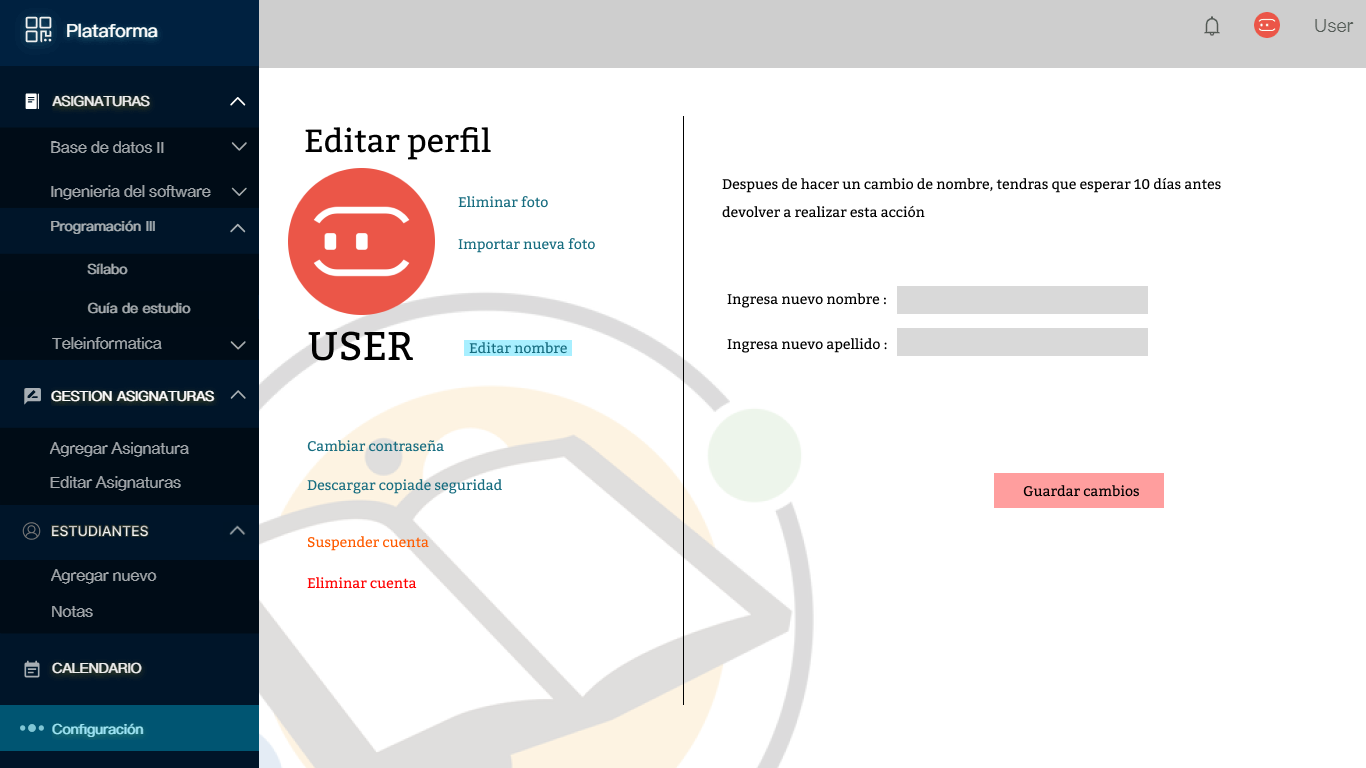
\includegraphics[scale=0.40]{20.png}
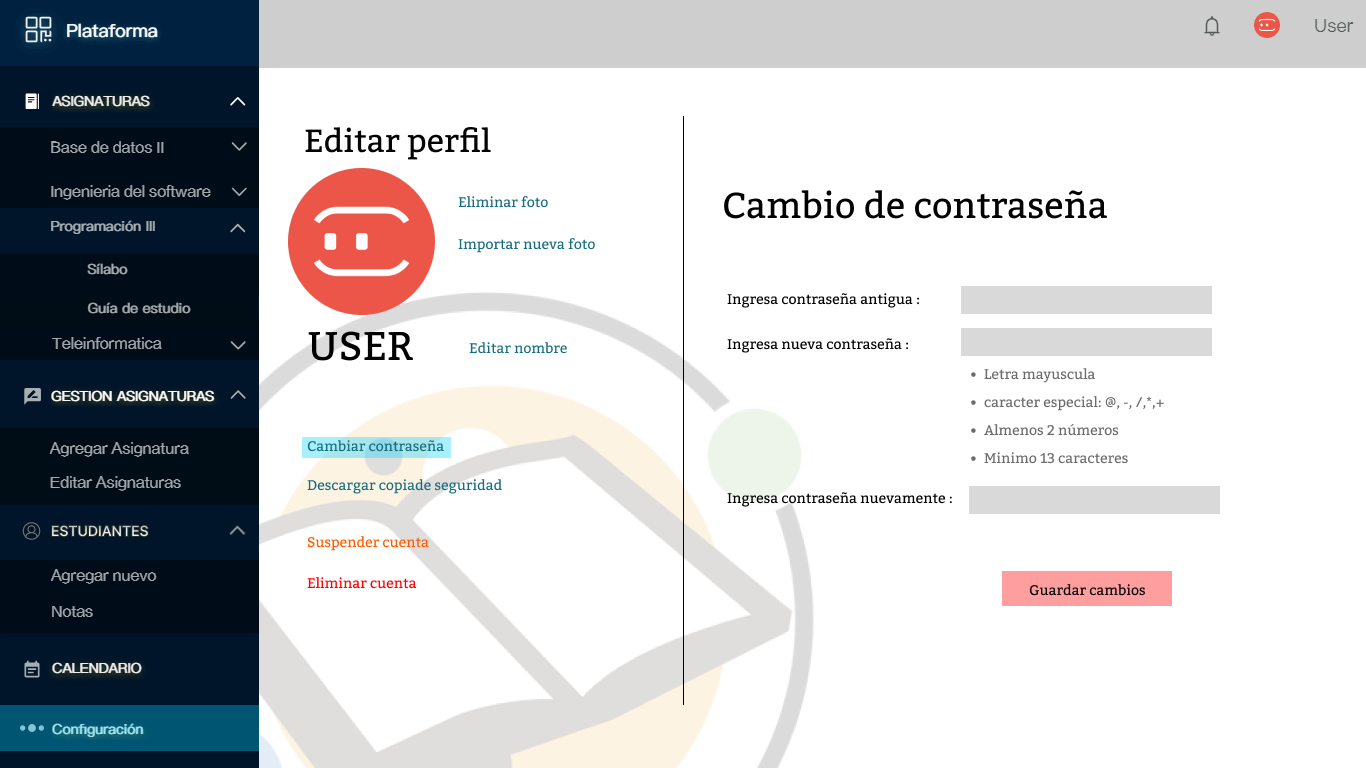
\includegraphics[scale=0.40]{21.png}
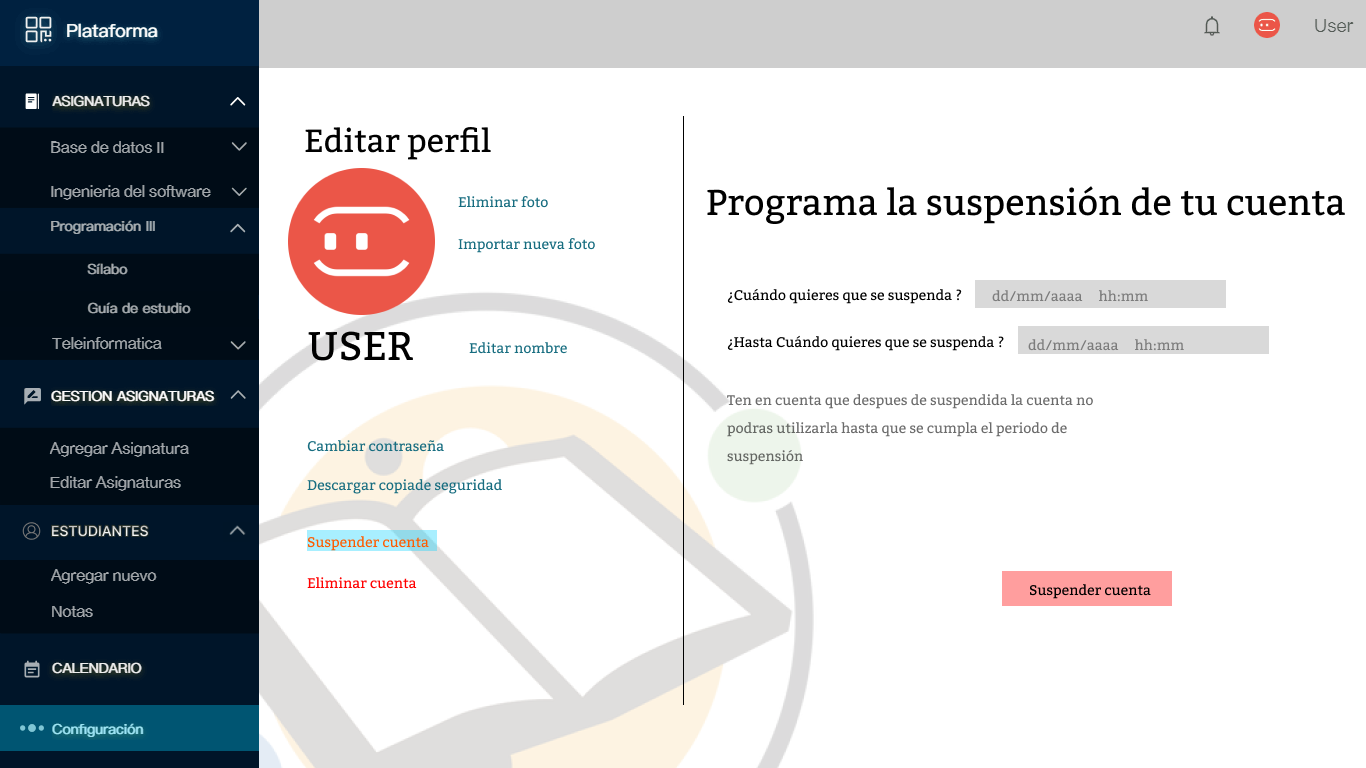
\includegraphics[scale=0.40]{22.png}
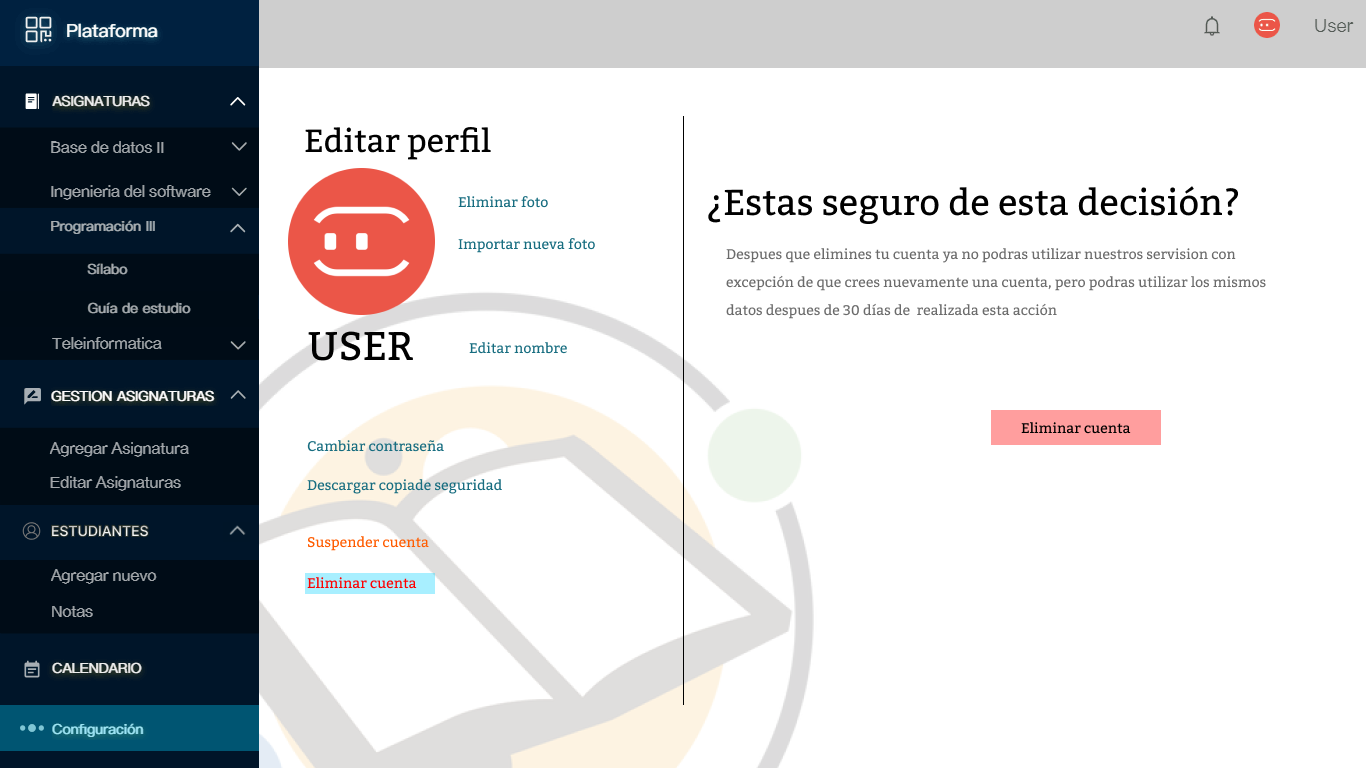
\includegraphics[scale=0.40]{23.png}
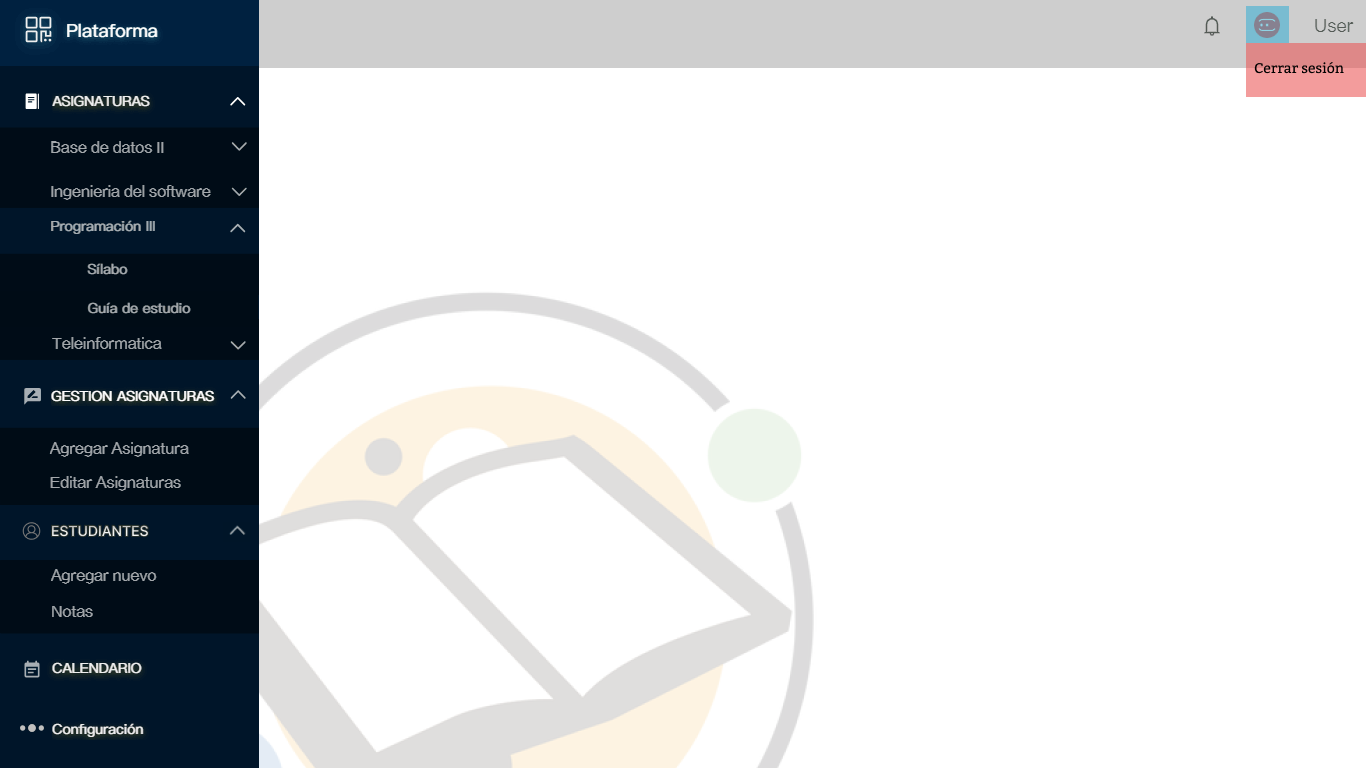
\includegraphics[scale=0.40]{24.png}
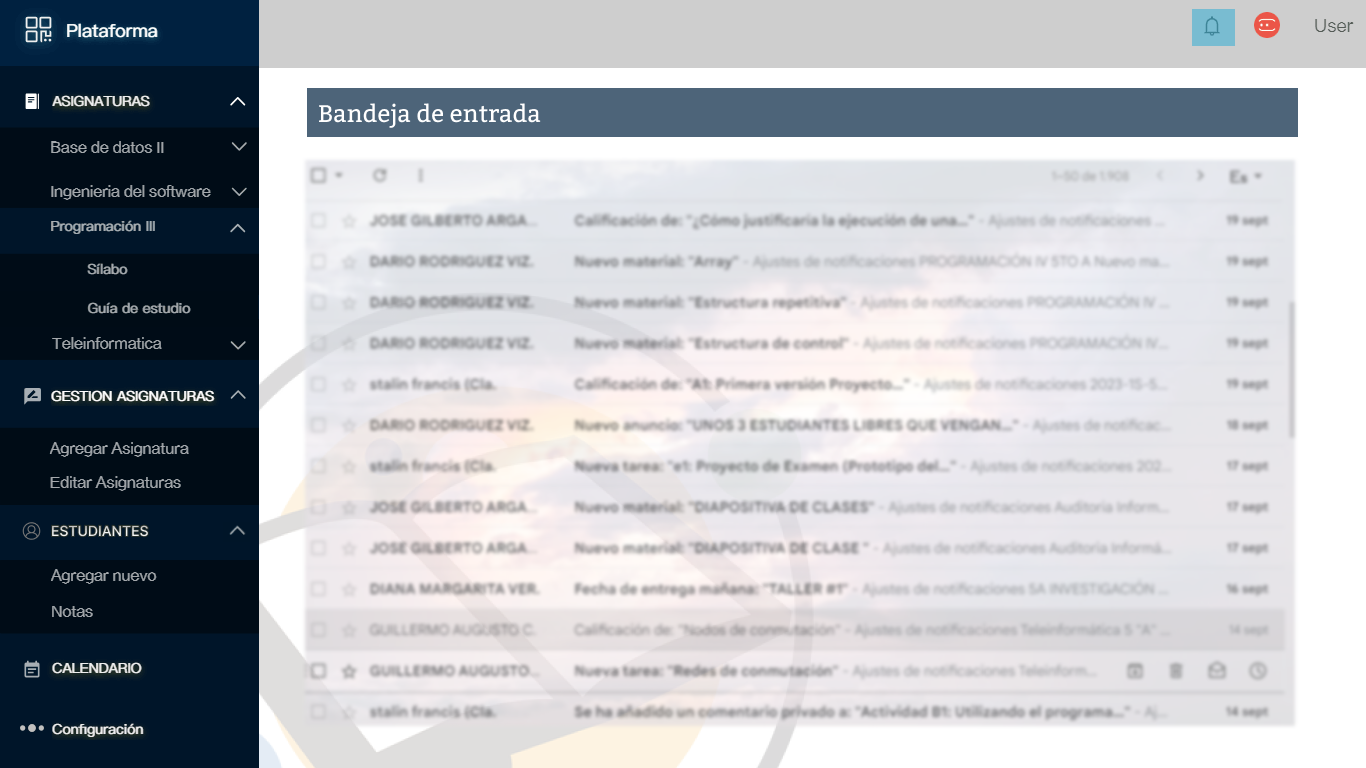
\includegraphics[scale=0.40]{25.png}
\newpage

\vspace{2cm} 
\begin{center}
\Huge 
\textbf{ESPECIFICACIÓN DE REQUISITOS DE SOFTWARE
PROYECTO AUTOMATIZACIÓN GESTION DE
ASIGNATURAS}
\end{center}

\newpage

\Huge
\textbf{Ficha del documento}
\vspace{7cm}

\normalsize

\begin{tabular}{|c|c|c|c|}
\hline
Fecha & Revisión & Líder del Proyecto & Verificación del Proyecto \\
\hline
\multirow{8}{}{20/10/2023} & \multirow{8}{}{1.1} & \multirow{8}{}{Ulloa Mina Alber Dayan} & \multirow{8}{}{ING.Stalin Francis} \\
& & & \\
& & & \\
& & & \\
& & & \\
& & & \\
& & & \\
& & & \\
\hline
\end{tabular}

\newpage


\section{\textbf{Introducción}}

Este documento es una Especificación de Requisitos de Software (ERS)
para el Sistema de Gestión de Asignaturas. La estructura de esta 
especificación se basa en las directrices proporcionadas por el
estándar IEEE Práctica Recomendada para Especificaciones de 
Requisitos de Software ANSI/IEEE 830, 1998.

\subsection{\textbf{Propósito}}

El propósito de este documento es definir las especificaciones 
funcionales y no funcionales para el desarrollo de un sistema de
gestión de asignaturas, el cual será utilizado por instituciones
educativas, profesores y estudiantes. Este sistema tiene como
objetivo principal facilitar la gestión eficiente de asignaturas,
incluyendo la planificación, la comunicación y la evaluación.

\subsection{\textbf{Alcance}}

Esta especificación de requisitos está dirigida a usuarios y 
administradores del sistema de gestión de asignaturas. El sistema se 
enfoca en la gestión de asignaturas en el ámbito educativo, lo que 
incluye la planificación de programas académicos, la comunicación 
entre profesores y estudiantes, y la evaluación del desempeño 
académico. El software permitirá una gestión efectiva de las 
asignaturas, promoviendo un entorno de aprendizaje enriquecedor y 
eficiente.
\subsection{\textbf{Personal involucrado}}
\vspace{10pt}

\begin{tabular}{|c|c|}

\hline
Nombre & Alber Dayan Ulloa Mina  \\
\hline
Rol & Analista, arquitecto y desarrollador de software \\
\hline
Responsabilidad & Análisis de información, arquitectura y programación del Software  \\
\hline
Información de contacto & alber.ulloa.mina@utelvt.edu.ec \\
\hline

\end{tabular}

\vspace{10pt}

\begin{tabular}{|c|c|}

\hline
Nombre & Alex Junior Añapa San Nicolas  \\
\hline
Rol & Analista, arquitecto y desarrollador de software \\
\hline
Responsabilidad & Análisis de información, arquitectura y programación del Software  \\
\hline
Información de contacto & alex.anapa.sannicolas@utelvt.edu.ec \\
\hline

\end{tabular}
\vspace{10pt}

\begin{tabular}{|c|c|}

\hline
Nombre & Belgica Jurany Perea Ramos  \\
\hline
Rol & Analista, arquitecto y desarrollador de software \\
\hline
Responsabilidad & Análisis de información, arquitectura y programación del Software  \\
\hline
Información de contacto & belgica.perea@utelvt.edu.ec \\
\hline

\end{tabular}
\vspace{10pt}

\begin{tabular}{|c|c|}

\hline
Nombre & Angélica Quintero Alcivar  \\
\hline
Rol & Analista, arquitecto y desarrollador de software \\
\hline
Responsabilidad & Análisis de información, arquitectura y programación del Software  \\
\hline
Información de contacto & angelica.quintero.alcivar@utelvt.edu.ec \\
\hline

\end{tabular}
\vspace{10pt}

\begin{tabular}{|c|c|}

\hline
Nombre & Leah Del Carmen Ayoví Ramos \\
\hline
Rol & Analista, arquitecto y desarrollador de software \\
\hline
Responsabilidad & Análisis de información, arquitectura y programación del Software  \\
\hline
Información de contacto & lia.ayovi.ramos@utelvt.edu.ec \\
\hline

\end{tabular}
\vspace{10pt}

\begin{tabular}{|c|c|}

\hline
Nombre & Pianina Zambrano  \\
\hline
Rol & Analista, arquitecto y desarrollador de software \\
\hline
Responsabilidad & Análisis de información, arquitectura y programación del Software  \\
\hline
Información de contacto & pianina.zambrano@utelvt.edu.ec \\
\hline

\end{tabular}
\subsection{\textbf{Definiciones, acrónimos y abreviaturas}}

\vspace{10pt}

\begin{tabular}{|c|c|}

\hline
\textit{Nombre} & \textit{Descripción}  \\
\hline
Usuario & Persona que usará el sistema para gestionar asignaturas \\
\hline
SGAI & Sistema de Gestión de Asignaturas Integrado \\
\hline
ERS & Especificación de Requisitos Software \\
\hline
RF & Requerimiento Funcional \\
\hline
RNF & Requerimiento No Funcional\\
\hline
FEE & Factibilidad, exactitud y eficacia \\
\hline

\end{tabular}

\subsection{\textbf{Referencias}}

\begin{tabular}{|c|c|}

\hline
\textit{Título de documento} & \textit{Referencias}  \\
\hline
Standard IEEE 830 - 1998 & IEEE-830 \\
\hline

\end{tabular}


\newpage

\subsection{\textbf{Resumen}}

Este documento sobre el software de gestión de asignaturas consta 
principalmente de tres secciones fundamentales. En la primera
sección, se presenta una introducción que ofrece una visión general
de la especificación de requisitos del software de gestión de 
asignaturas.
La segunda sección se dedica a una descripción global del sistema,
donde se detallan minuciosamente las funcionalidades del software
para la gestión de asignaturas, además de los recursos necesarios
para su ejecución eficiente. Este análisis exhaustivo del sistema es
crucial, ya que sienta las bases antes de la creación del software 
de gestión de asignaturas.
En la tercera sección, se establecen con precisión los requisitos, 
tanto directos como indirectos, que el sistema de gestión de 
asignaturas debe cumplir para su uso adecuado. Estos requisitos son 
fundamentales para asegurar la factibilidad, precisión y eficacia
del software durante su uso continuado en el ámbito educativo.

\section{\textbf{Descripción general}}

\subsection{\textbf{Descripción del producto}}

Al completar el desarrollo del software de gestión de asignaturas, y
ejecutarse, proporcionará a los usuarios una interfaz organizada y
eficiente para gestionar y acceder a los datos de asignaturas, 
incluyendo planes de estudio, comunicaciones y evaluaciones. La 
interfaz reflejará de manera precisa y coherente la estructura y la 
información tal y como se ha diseñado en la codificación del 
software.

\subsection{\textbf{Funcionalidad del Software}}

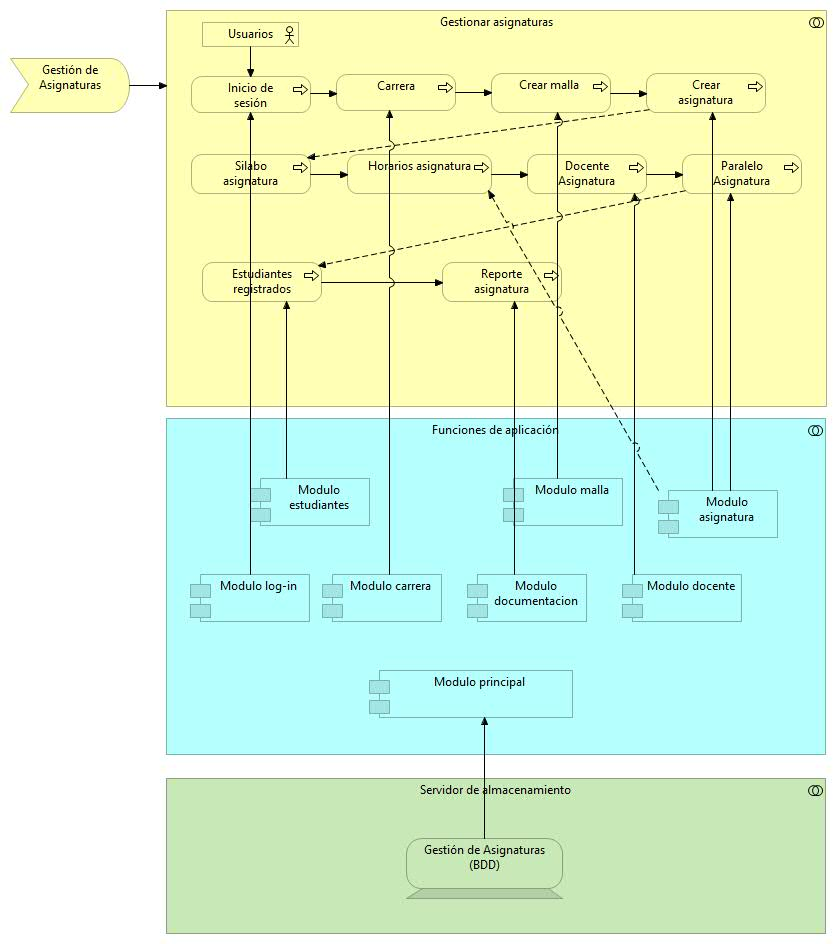
\includegraphics[scale=0.65]{ModelG.A.jpg}

\subsection{\textbf{Características de los usuarios}}

\vspace{10pt}

\begin{tabular}{|c|c|}

\hline
Tipo de usuario  & Usuario del Software \\
\hline
Formación & Universitaria \\
\hline
Actividades & Monitorización y gestión de Asignaturas  \\
\hline

\end{tabular}

\subsection{\textbf{Restricciones}}

\begin{enumerate}
\item Software desarrollado para sistema operativo windows 7 en 
adelante
\item  Lenguajes y tecnologías en uso: Java, PHPMyAdmin.
\item  El sistema deberá tener un diseño e implementación sencilla.
\end{enumerate}

\subsection{\textbf{Suposiciones y dependencias}}
\begin{enumerate}
\item Se asume que los requisitos aquí descritos son estables.
\item Los equipos en los que se vaya a ejecutar el sistema deben
cumplir los requisitos antes indicados para garantizar una ejecución
correcta de la misma.
\end{enumerate}

\section{\textbf{Descripción general}}

\subsection{\textbf{Requerimientos Funcionales}}


\vspace{15pt}

\begin{tabular}{|c|c|} 
\hline
\textbf{Identificación del requerimiento:} & RF01  \\
\hline
\textbf{Nombre del Requerimiento}: & Visualizar el contenido de cada 
una de las asignaturas \\
\hline
\textbf{Características:} & Permitirá únicamente la visualización de 
todas las tareas y \\ & actividades que se carguen en una asignatura
específica.  \\
\hline
\textbf{Descripción del requerimiento:} & El sistema podrá brindar 
datos de visualización\\ & al usuario autorizado para que constate 
la actividad de las asignaturas \\
\hline
\textbf{Requerimiento NO funcional:} & RNF01 \\
& RNF04  \\
\hline
\textbf{Prioridad de requerimiento:} & Alta \\
\hline

\end{tabular}



\vspace{15pt}

\begin{tabular}{|c|c|} 
\hline
\textbf{Identificación del requerimiento:} & RF02  \\
\hline
\textbf{Nombre del Requerimiento}: &Visualizar Guía de estudio y 
Sílabo \\
\hline
\textbf{Características:} & Permitirá únicamente la visualización de
la guía de  estudio y el\\ & sílabo que  se carguen en una 
asignatura específica.  \\
\hline
\textbf{Descripción del requerimiento:} & El sistema podrá brindar 
datos de visualización al \\ & usuario autorizado para que 
monitorice si los documentos cargados \\ & en esa asignatura son los 
adecuados \\
\hline
\textbf{Requerimiento NO funcional:} & RNF01 \\
\hline
\textbf{Prioridad de requerimiento:} & Alta \\
\hline

\end{tabular}


\vspace{15pt}

\begin{tabular}{|c|c|} 
\hline
\textbf{Identificación del requerimiento:} & RF03  \\
\hline
\textbf{Nombre del Requerimiento}: & Agregar asignatura nueva \\
\hline
\textbf{Características:} & Le brindará al usuario un formulario que
deberá llenar  con \\ & los datos de la nueva asignatura que desea 
agregar  \\
\hline
\textbf{Descripción del requerimiento:} & Permitirá que el 
administrador de Asignaturas añada  una\\ & asignatura  nueva dentro
del sistema educativo \\
\hline
\textbf{Requerimiento NO funcional:} & RNF01 \\
& RNF04  \\
\hline
\textbf{Prioridad de requerimiento:} & Alta \\
\hline

\end{tabular}


\vspace{15pt}

\begin{tabular}{|c|c|} 
\hline
\textbf{Identificación del requerimiento:} & RF04  \\
\hline
\textbf{Nombre del Requerimiento}: & Editar asignatura \\
\hline
\textbf{Características:} & Le brinda al usuario el formulario 
necesario para editar los datos de \\ &una asignatura ya agregada \\
\hline
\textbf{Descripción del requerimiento:} & Por medio de un formulario
se cargan los datos ya registrados en\\ & una asignatura específica
con la posibilidad de editar los mismos \\
\hline
\textbf{Requerimiento NO funcional:} & RNF01  \\
\hline
\textbf{Prioridad de requerimiento:} & Alta \\
\hline

\end{tabular}

\vspace{15pt}

\begin{tabular}{|c|c|} 
\hline
\textbf{Identificación del requerimiento:} & RF05  \\
\hline
\textbf{Nombre del Requerimiento}: & Eliminación de estudiantes \\
\hline
\textbf{Características:} & Le otorgará privilegios al usuario para
eliminar los estudiantes \\ & ue se encuentren matriculados en una 
asignatura \\
\hline
\textbf{Descripción del requerimiento:} & Mediante una previa 
consulta de los estudiantes\\ & que se encuentren matriculados en
una determinada \\ &  asignatura el usuario podrá eliminar \\
\hline
\textbf{Requerimiento NO funcional:} & RNF01 \\
& RNF02  \\
\hline
\textbf{Prioridad de requerimiento:} & Alta \\
\hline

\end{tabular}


\vspace{15pt}

\begin{tabular}{|c|c|} 
\hline
\textbf{Identificación del requerimiento:} & RF06  \\
\hline
\textbf{Nombre del Requerimiento}: & Agregar nuevo estudiante a 
asignatura \\
\hline
\textbf{Características:} & Permitirá que el usuario agregue un 
nuevo \\ & estudiante en una determinada asignatura \\
\hline
\textbf{Descripción del requerimiento:} & Mediante una previa
consulta de los estudiantes que\\ & se encuentren registrados en el
plantel educativo, \\ &  el usuario podrá agregarlos a cualquier 
asignatura que desee \\
\hline
\textbf{Requerimiento NO funcional:} & RNF01 \\
& RNF02  \\
\hline
\textbf{Prioridad de requerimiento:} & Alta \\
\hline

\end{tabular}


\vspace{15pt}

\begin{tabular}{|c|c|} 
\hline
\textbf{Identificación del requerimiento:} & RF07  \\
\hline
\textbf{Nombre del Requerimiento}: & Eliminación de estudiantes \\
\hline
\textbf{Características:} & Le otorgará privilegios al usuario para 
eliminar los estudiantes \\ &que se encuentren matriculados en una
asignatura \\
\hline
\textbf{Descripción del requerimiento:} & Mediante una previa 
consulta de los estudiantes que se\\ & encuentren matriculados en
una determinada \\ &  asignatura el usuario podrá eliminar \\
\hline
\textbf{Requerimiento NO funcional:} & RNF01 \\
& RNF03  \\
\hline
\textbf{Prioridad de requerimiento:} & Alta \\
\hline

\end{tabular}


\vspace{15pt}

\begin{tabular}{|c|c|} 
\hline
\textbf{Identificación del requerimiento:} & RF08  \\
\hline
\textbf{Nombre del Requerimiento}: & Configuración del perfil de
usuario \\
\hline
\textbf{Características:} & Permitirá que se modifiquen datos de los 
perfiles autorizados \\ & para esta gestión de asignaturas \\
\hline
\textbf{Descripción del requerimiento:} & Le otorgará al usuario el
privilegio de editar \\ &los datos personales de su perfil como 
nombre, foto, contraseña, \\ & o descargar una copia de seguridad \\
\hline
\textbf{Requerimiento NO funcional:} & RNF01 \\
\hline
\textbf{Prioridad de requerimiento:} & Alta \\
\hline

\end{tabular}

\subsection{\textbf{Requerimientos No Funcionales}}

\vspace{15pt}

\begin{tabular}{|c|c|} 
\hline
\textbf{Identificación del requerimiento:} & RNF01  \\
\hline
\textbf{Nombre del Requerimiento}: & Interfaz sencilla e intuitiva
para el usuario \\
\hline
\textbf{Características:} & Interfaz sencilla e intuitiva para el
usuario\\ & para que sea de fácil manejo a los usuarios del sistema.
\\
\hline
\textbf{Descripción del requerimiento:} & El sistema debe tener una
interfaz de uso intuitiva y sencilla.  \\
\hline
\textbf{Prioridad de requerimiento:} & Alta \\
\hline

\end{tabular}


\vspace{15pt}

\begin{tabular}{|c|c|} 
\hline
\textbf{Identificación del requerimiento:} & RNF02  \\
\hline
\textbf{Nombre del Requerimiento}: & Consulta de Estudiantes \\
\hline
\textbf{Características:} & Permite que el usuario consulte los
estudiantes\\
\hline
\textbf{Descripción del requerimiento:} & Mediante un pequeño
formulario el software permite lque el usuario \\ & pueda consultar
desde la  base de datos los  estudiantes matriculados \\
\hline
\textbf{Prioridad de requerimiento:} & Alta \\
\hline

\end{tabular}

\vspace{15pt}

\begin{tabular}{|c|c|} 
\hline
\textbf{Identificación del requerimiento:} & RNF03  \\
\hline
\textbf{Nombre del Requerimiento}: & Notas de los estudiantes \\
\hline
\textbf{Características:} & Permite que se genere un reporte de las
notas de los estudiantes \\ & matriculados en una asignatura 
especifica.\\
\hline
\textbf{Descripción del requerimiento:} & Mediante un pequeño
formulario el software permite  que el usuario\\ & pueda consultar
desde la base de datos  las notas\\ & de los estudiantes 
matriculados en una asignatura especifica \\
\hline
\textbf{Prioridad de requerimiento:} & Alta \\
\hline

\end{tabular}

\vspace{15pt}

\begin{tabular}{|c|c|} 
\hline
\textbf{Identificación del requerimiento:} & RNF04  \\
\hline
\textbf{Nombre del Requerimiento}: & Calendario académico \\
\hline
\textbf{Características:} & Otorga información sobre las fechas establecidas para las tareas y \\ & actividades de las asignaturas.\\
\hline
\textbf{Descripción del requerimiento:} & En el calendario se reflejará con fecha exacta las actividades de cada\\ & asignatura, como tareas, y eventos educativos. \\
\hline
\textbf{Prioridad de requerimiento:} & Alta \\
\hline

\end{tabular}


\end{document} 



